\documentclass[12pt]{scrartcl}
\usepackage{geometry}
\usepackage{amsmath}
\usepackage[english]{babel}
\usepackage{fontspec}
\usepackage{hyperref}
\usepackage{subfigure}
\usepackage{framed}
\usepackage{float}
\usepackage[justification=RaggedRight, singlelinecheck=false]{caption}
\setmainfont{Fira Sans}
\geometry{a4paper,left=30mm,right=30mm, top=2cm, bottom=2cm}

\begin{document}
  \title{Project Work at MPIK}
  \subtitle{Temperature control system}
  \date{}
  \author{Stefan Dickopf}
  \maketitle

  \section{Introduction}
    During the 6 week project work the PID temperature control system in the
    control room of the THe-Trap experiment was to be developed further. A
    network communication was established using a Ethernet Shield on
    the Arduino Due platform which acts as the controller. Through this
    interface it is now possible to read out values and change the behaviour
    of the PID controller with a script running on a local machine.\\
    The level shifting circuit board for the in- and outputs on the Arduino
    was reconstructed into a sturdier design using SMD-parts on a milled
    circuit board.\\
    At last the temperature control was tested using the new network interface.

  \section{Experimental setup}
    A temperature sensor, a heater and a cooler are to be connected to a Arduino
    board. In order for it to work we need to have shifters for the voltage
    range to fit the inputs/outputs on the Arduino. This was first done by
    Vanessa Scheller using cables and a breadboard, I took her design and
    reworked it to be used on a milled circuit board and SMD parts.

    \subsection{Temperature sensor circuit}
      The circuit for the temperature sensor looks as follows:
      \begin{figure}[h]
        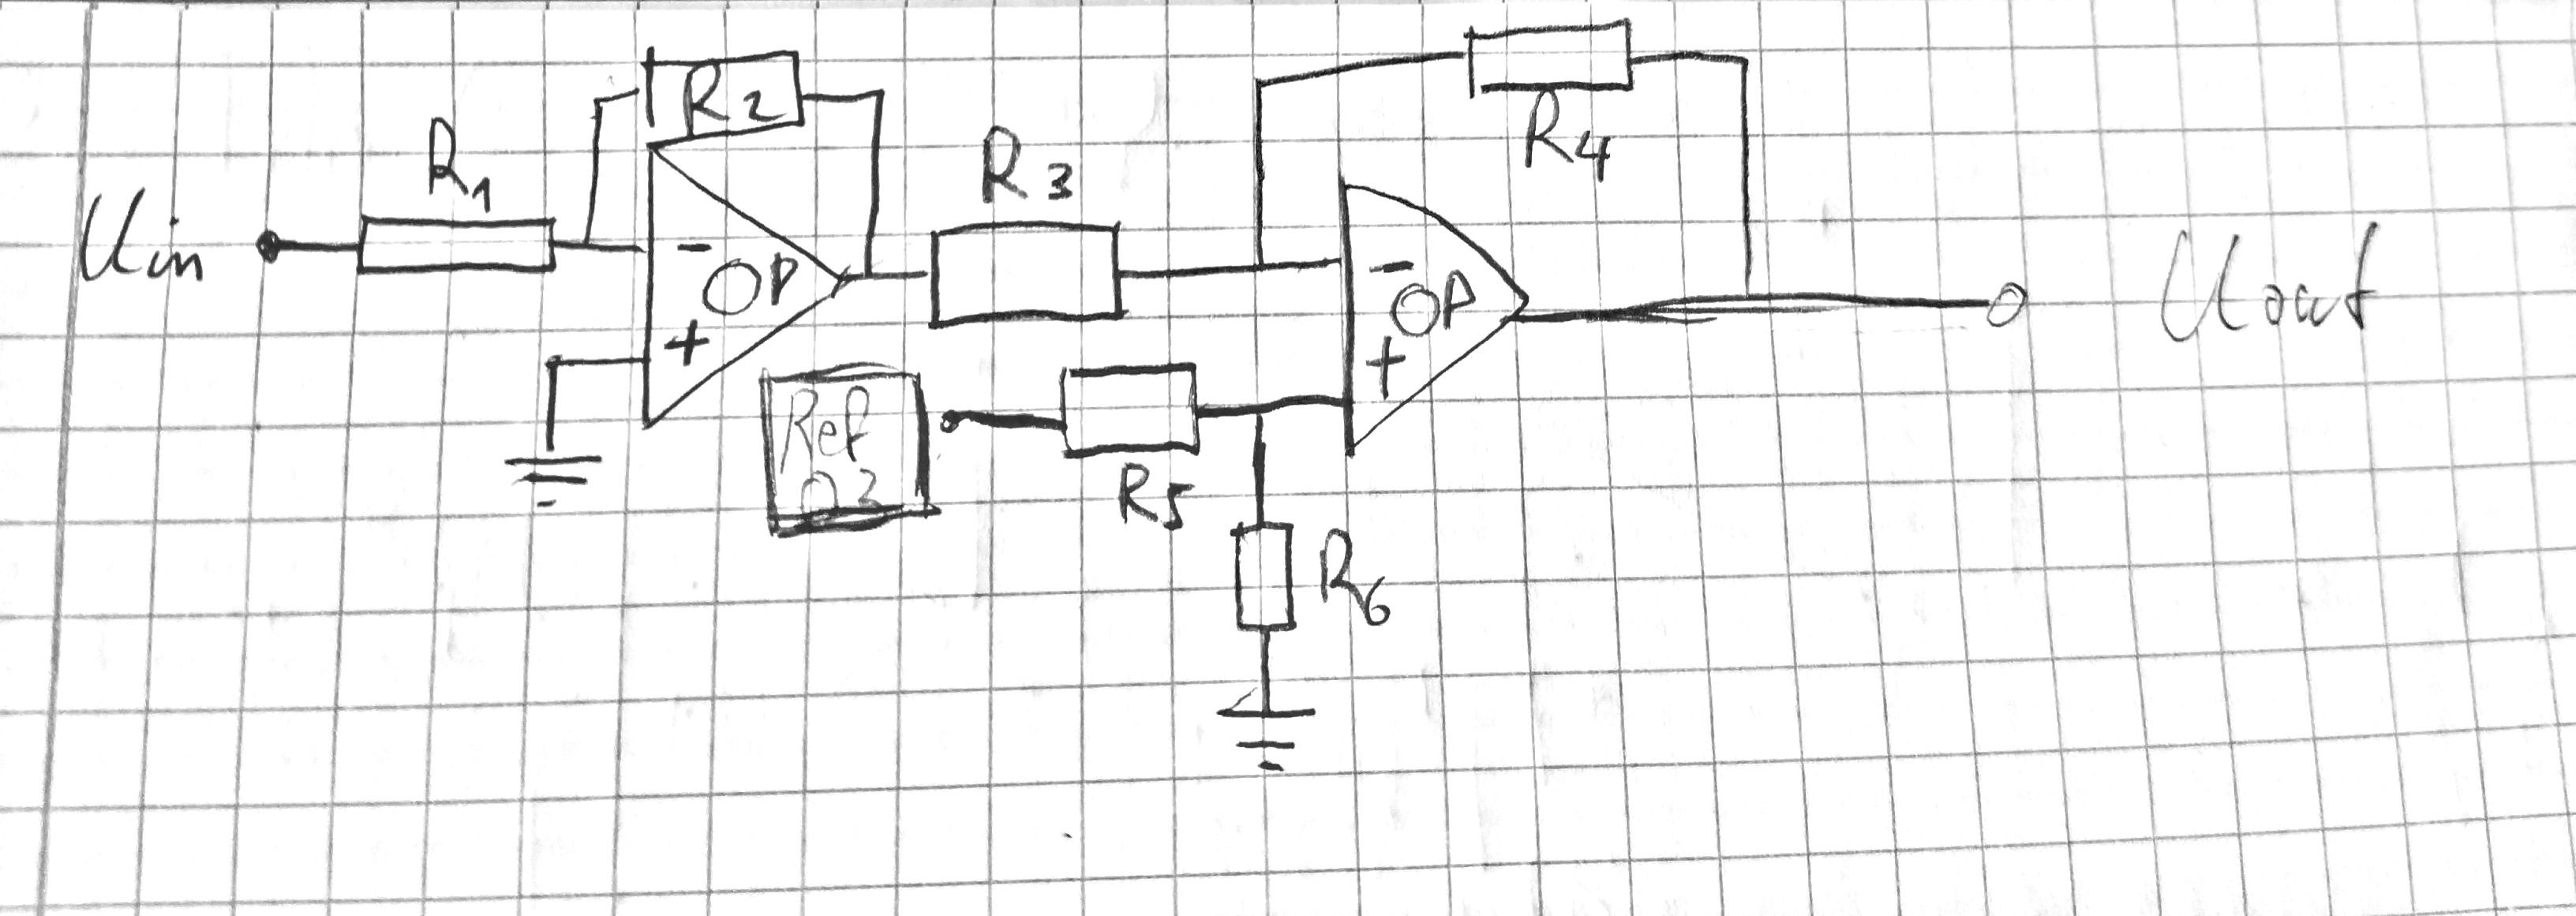
\includegraphics[width = \textwidth]{circ.png}
        \caption{Temp. sensor shifter circuit}
        \label{fig1}
      \end{figure}
      \\The input range from the temperature sensor we are interested in is
      $$-1.6 \, \text{V} < \text{U}_{\text{in}} < 1.6\, \text{V}$$
      The supply voltage of the op-amps is 15V. We want to have a cutoff after
      the first op-amp at the input range boundaries. This can be achieved with
      setting the amplification factor with $\text{R}_1$ and $\text{R}_2$. The output range
      should equal the input range of the Arduino analogue input which goes form
      0-3.3V. The values found for the resistances are as follows (the added value
      corresponds to a potentiometer in series): \\
      \begin{table}[H]\label{tempres}
        \begin{tabular}{l|c c c c c c}
          & $\text{R}_1$ & $\text{R}_2$ & $\text{R}_3$ & $\text{R}_4$
          & $\text{R}_5$ & $\text{R}_6$ \\
          \hline\vspace{5pt}
          $\text{R}[\text{k}\Omega]$ & $15$ & $133$ & $133$ & $12 + 5$ & $10$
          & $15 + 5$
        \end{tabular}
        \caption{Resistances for temp. shifter circuit}
      \end{table}
      This gives to following response to the input Voltage $U_{in}$\\
      \begin{figure}[h]
        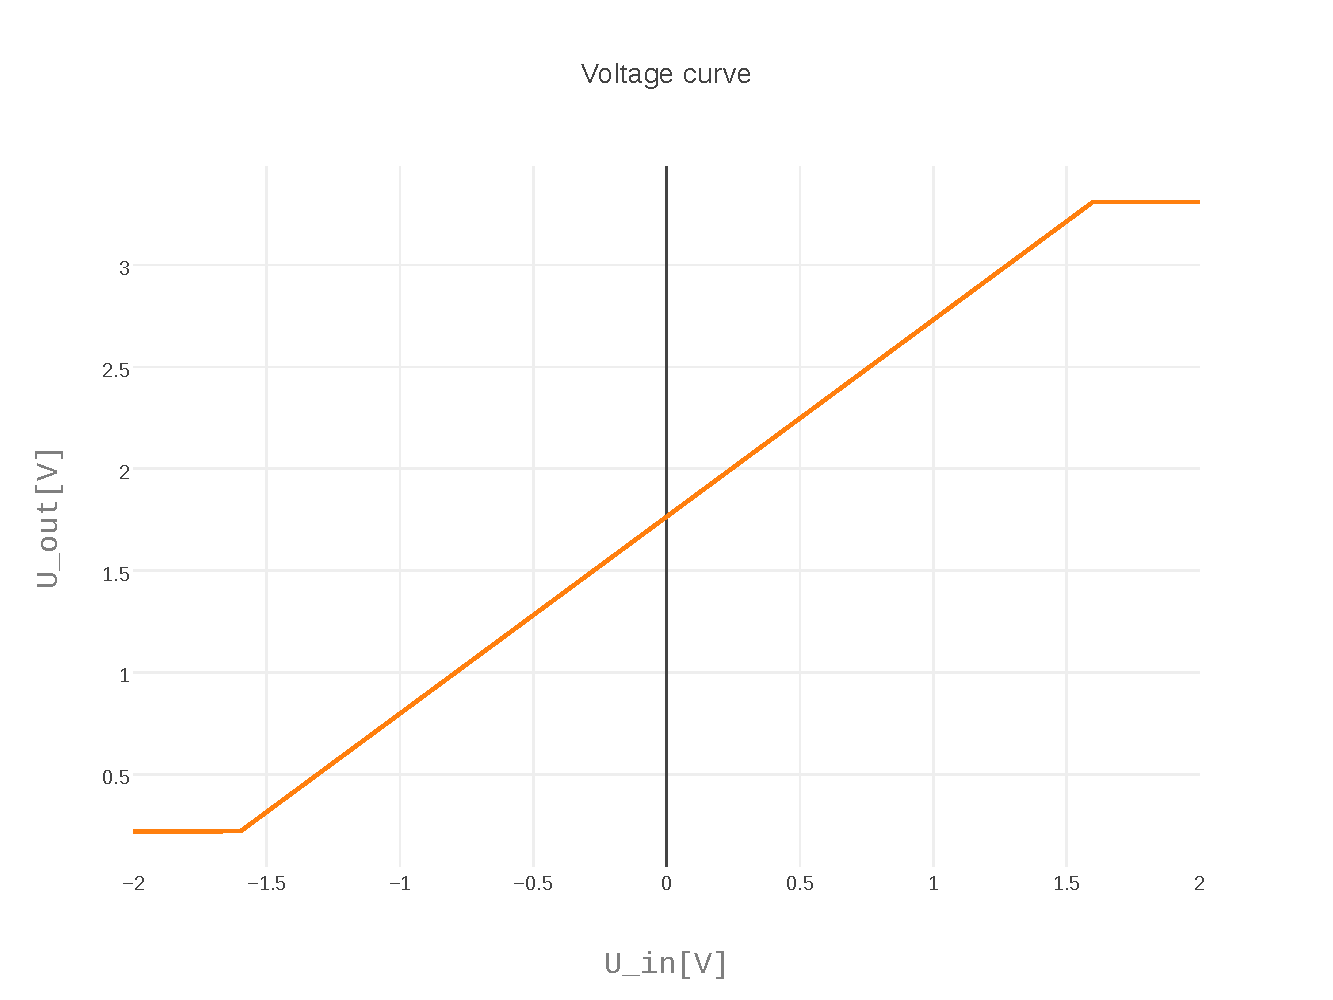
\includegraphics[width = \textwidth]{./plots/plot_image.pdf}
        \caption{Theoretical response of temp. shifter}
        \label{fig2}
      \end{figure}

    \subsection{Heater, cooler circuit}
      \begin{figure}[h]
        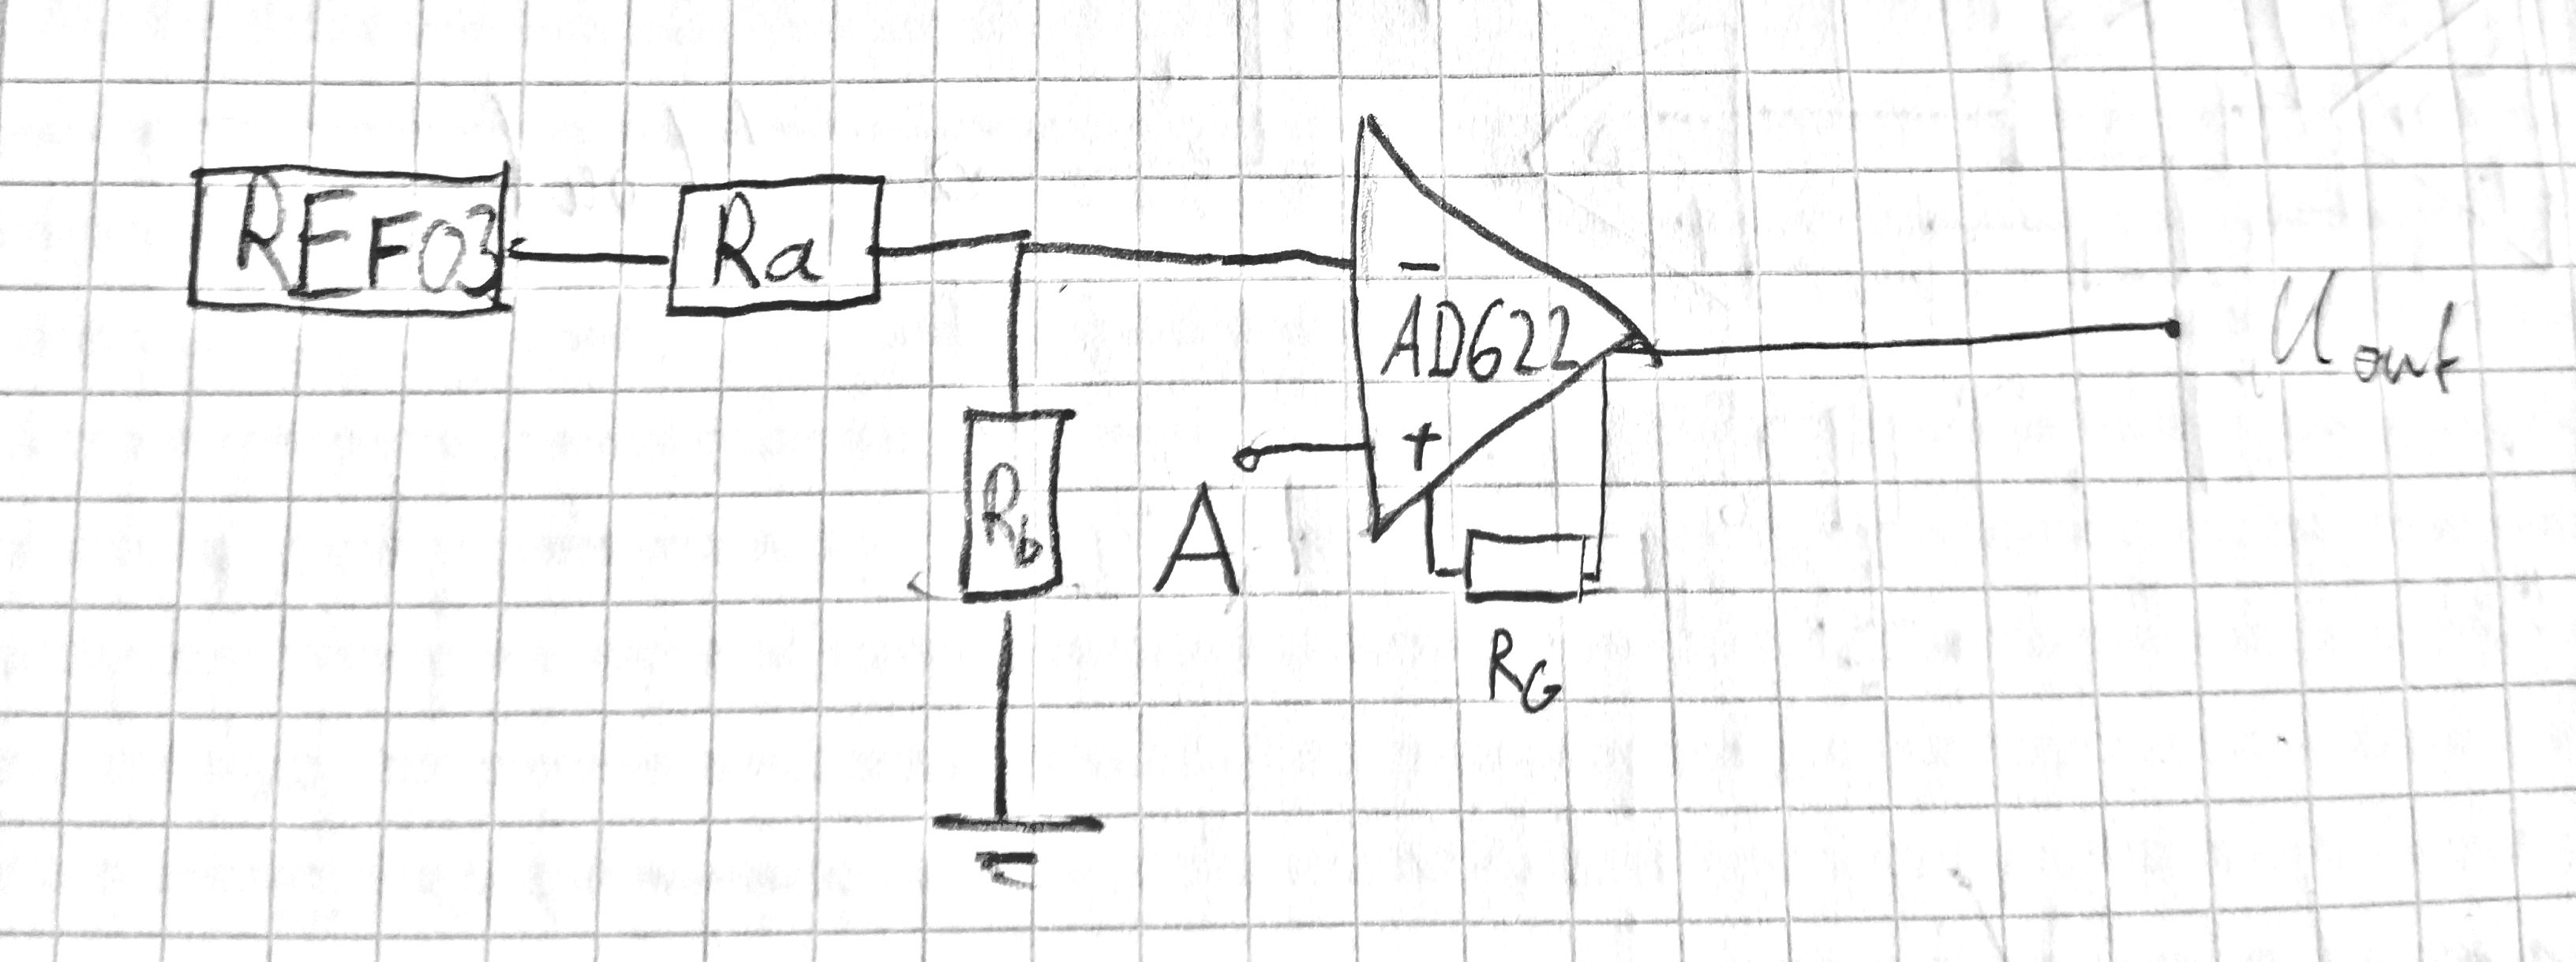
\includegraphics[width = \textwidth]{circ2.png}
        \caption{Heater/cooler shifter circuit}
        \label{fig3}
      \end{figure}
      The output range from the Arduino's DAC is $$0.55\, \text{V} <
      \text{U}_{\text{DAC}} < 2.75\, \text{V}$$
      The regulation voltage from the heater and cooler goes from 0 to 10V. First the
      voltage from the DAC output needs to be reduced by 0.55V and then amplified
      such that the maximum output from the DAC corresponds to the maximum input from
      the heater/cooler. The amplification is set with the resistance RG.
      The values found by Vanessa are: \\
      \begin{table}[H] \label{hcres}
        \begin{tabular}{l|c c c}
          & $\text{R}_\text{a}$ & $\text{R}_\text{b}$ & $\text{R}_\text{G}$ \\
          \hline\vspace{5pt}
          $\text{R}[\text{k}\Omega]$ & $3.92 + 5$ & $1$ & $27+10$
        \end{tabular}
        \flushleft \caption{Resistances for heater/cooler shifter circuit}
      \end{table}
      \noindent The output here can be described by the amplified difference of the two
      input voltages. The amplification factor was adjusted such that it gives
      the needed output range.
      To both circuits many capacitances are added, which are for filtering
      the input +15V/-15V and the ref03 voltages from AC voltage parts. This is done with
      10nF and 100nF capacitances in parallel.

    \subsection{Realization of the circuitboard}
      All of the circuits were realized using a SMD board. The circuitboard was
      constructed using EAGLE Professional and made with a circuit board cutter.
      It has the same proportions as the used Arduino Due, such that it fits
      into the enclosure thats already existing.
      \\The resistors and the capacitances are directly soldered onto the board,
      while the OP07 and the AD622 (not 620 as on the image) are put onto
      headers. The complete board is shown here in Figure~ \ref{fig5} and \ref{fig5}.
      \\ Notice that the header for the left AD622 was placed in the opposite
      direction, such that the marker for the top is actually on the other side
      than the top is supposed to be.\\
      Also some of the capacitances were not soldered in, on the design of the
      board they were made as a precaution.\\
      It was found that the heater/cooler cables add a capacitance which lead
      to oscillations on the temperature measurement. We added $100 \Omega$
      resistors on the heater/cooler output to resolve the issue.\\ In Figure~
      \ref{fig6} we see the board connected to the Arduino with the Ethernet
      Shield 2 on top.\\
      \begin{figure}[H]
        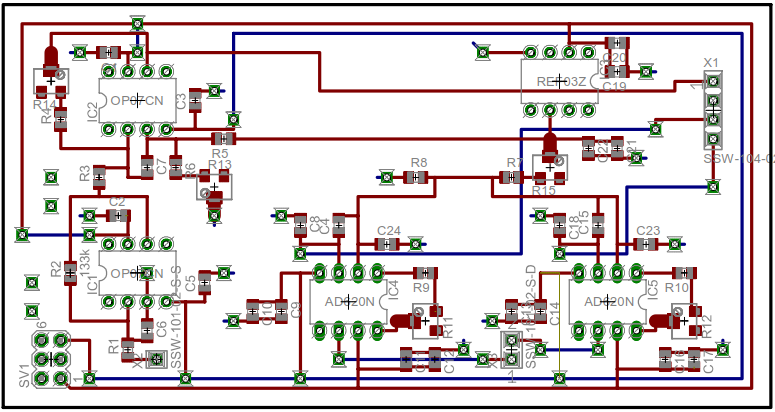
\includegraphics[width = \textwidth]{board.png}
        \caption{Circuitboard layout}
        \label{fig4}
      \end{figure}
      \begin{figure}[H]
        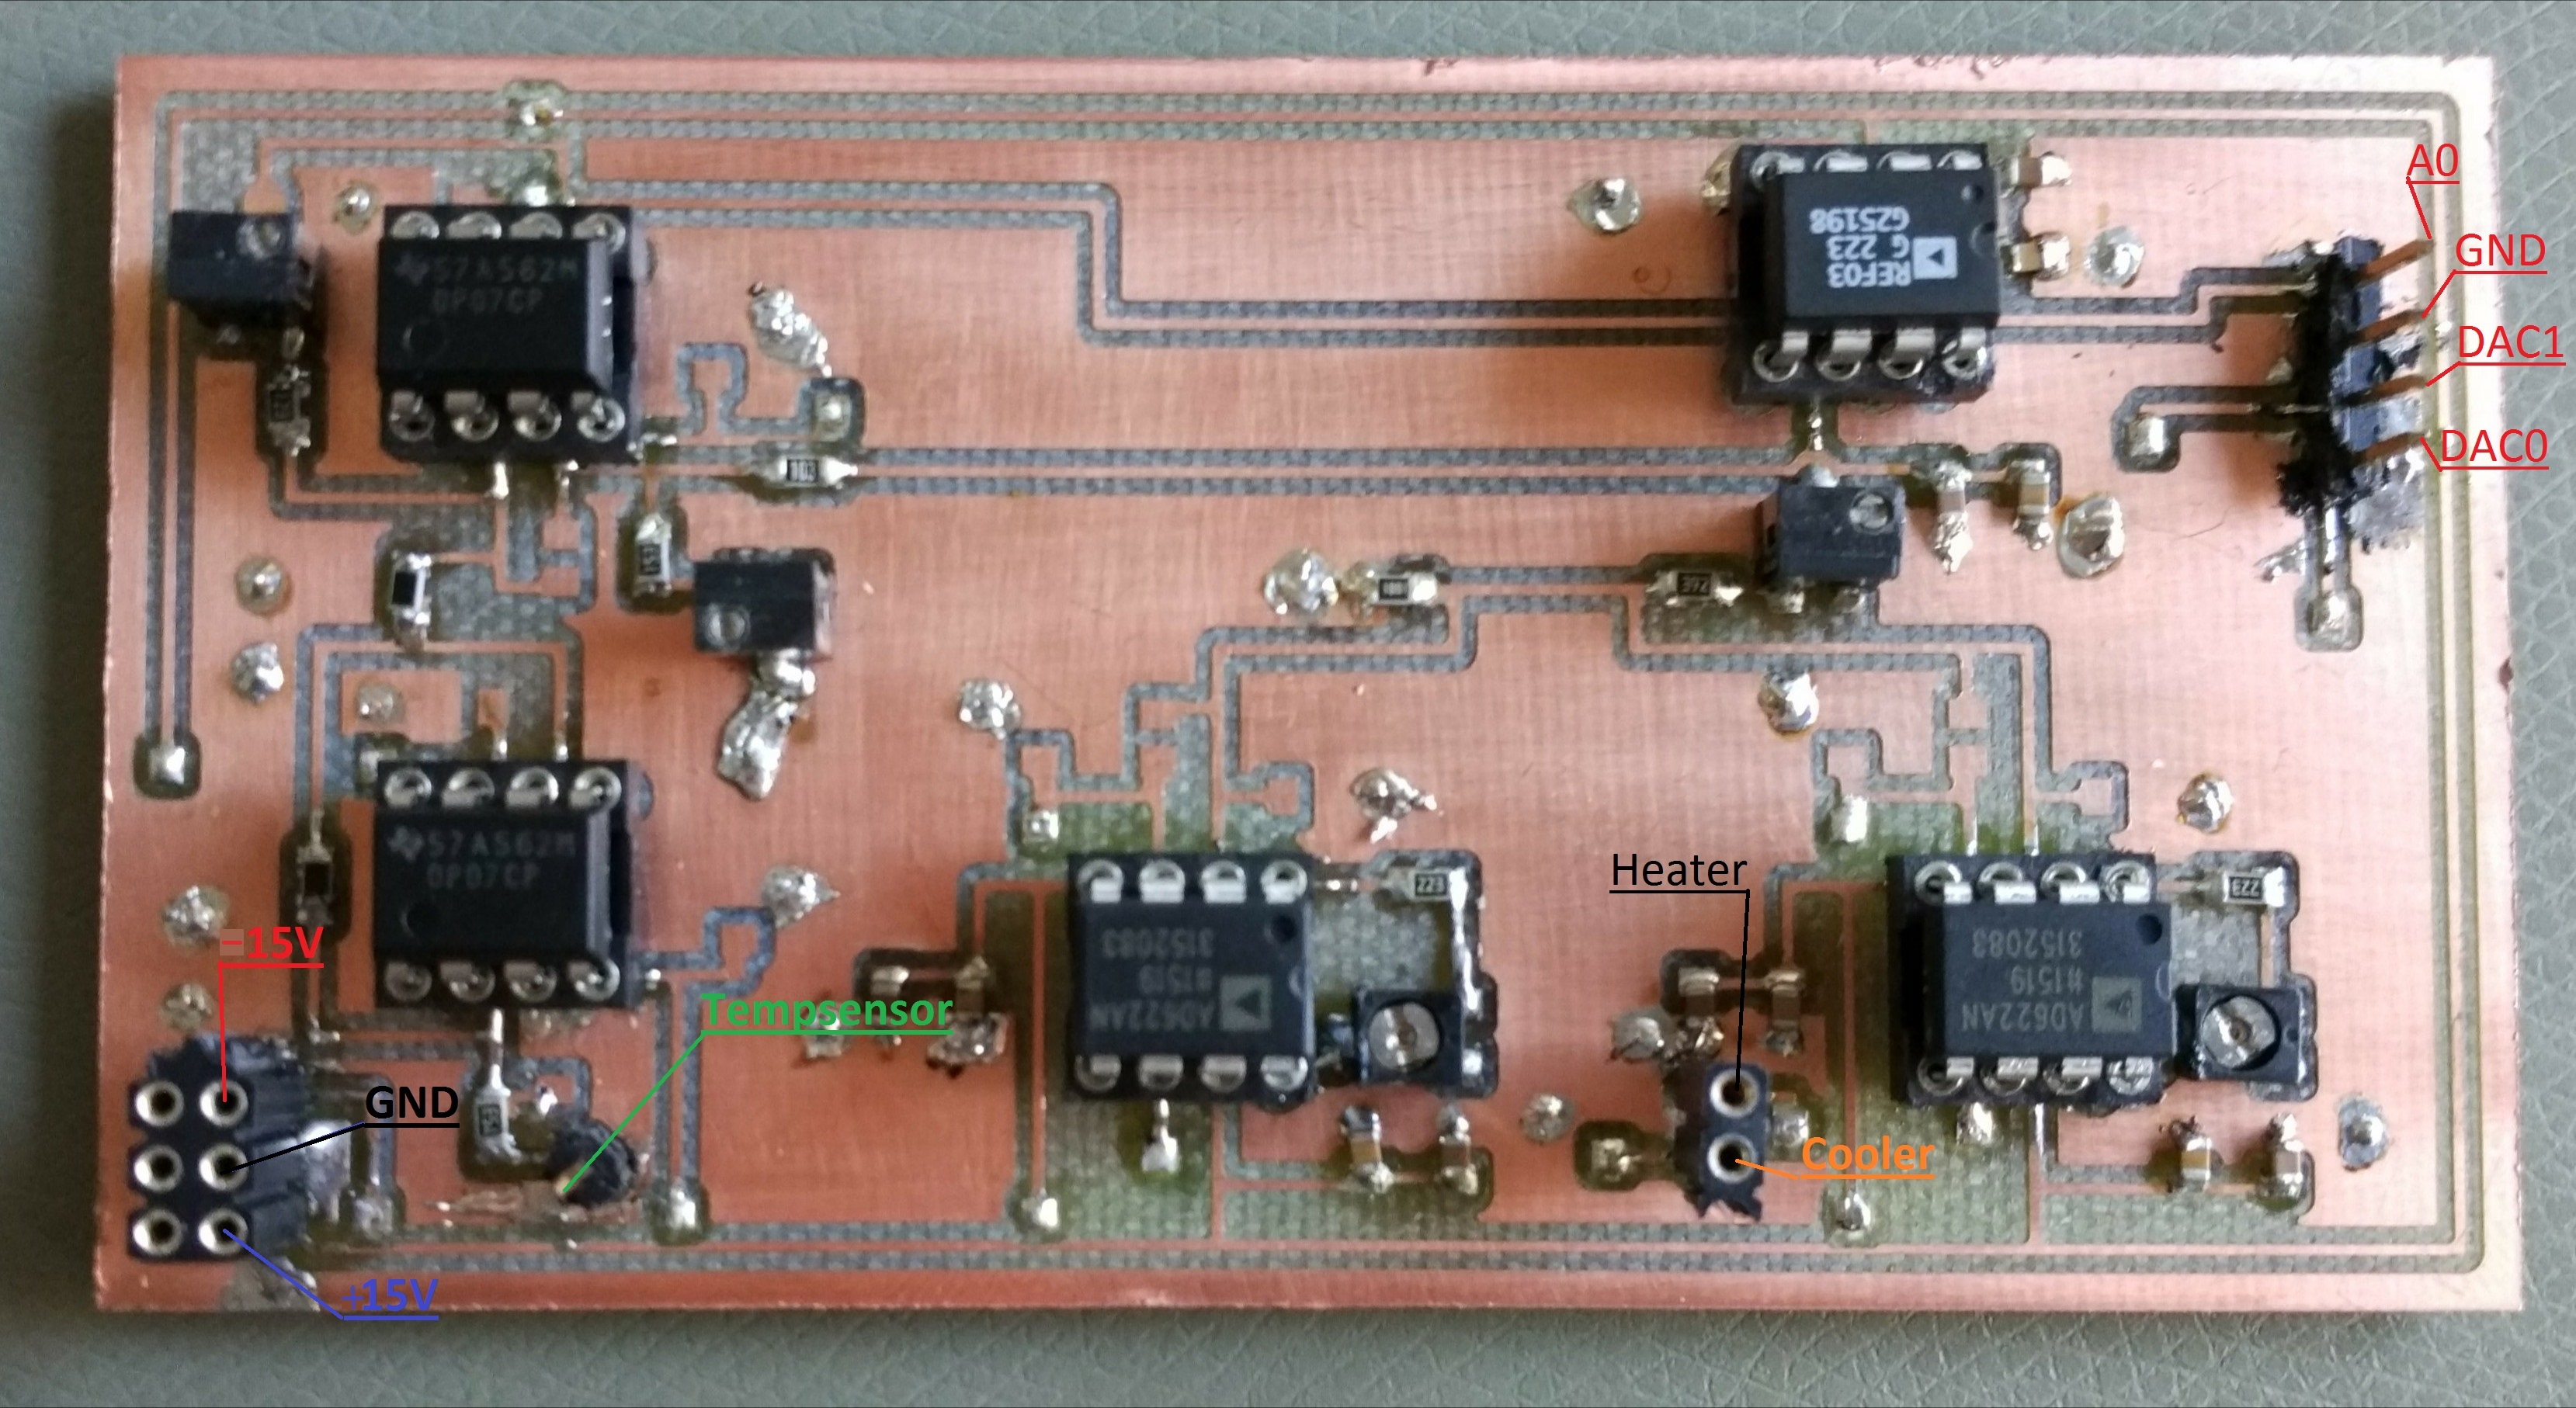
\includegraphics[width = \textwidth]{boardbild.jpg}
        \caption{Circuitboard picture}
        \label{fig5}
      \end{figure}
      \begin{figure}[H]
        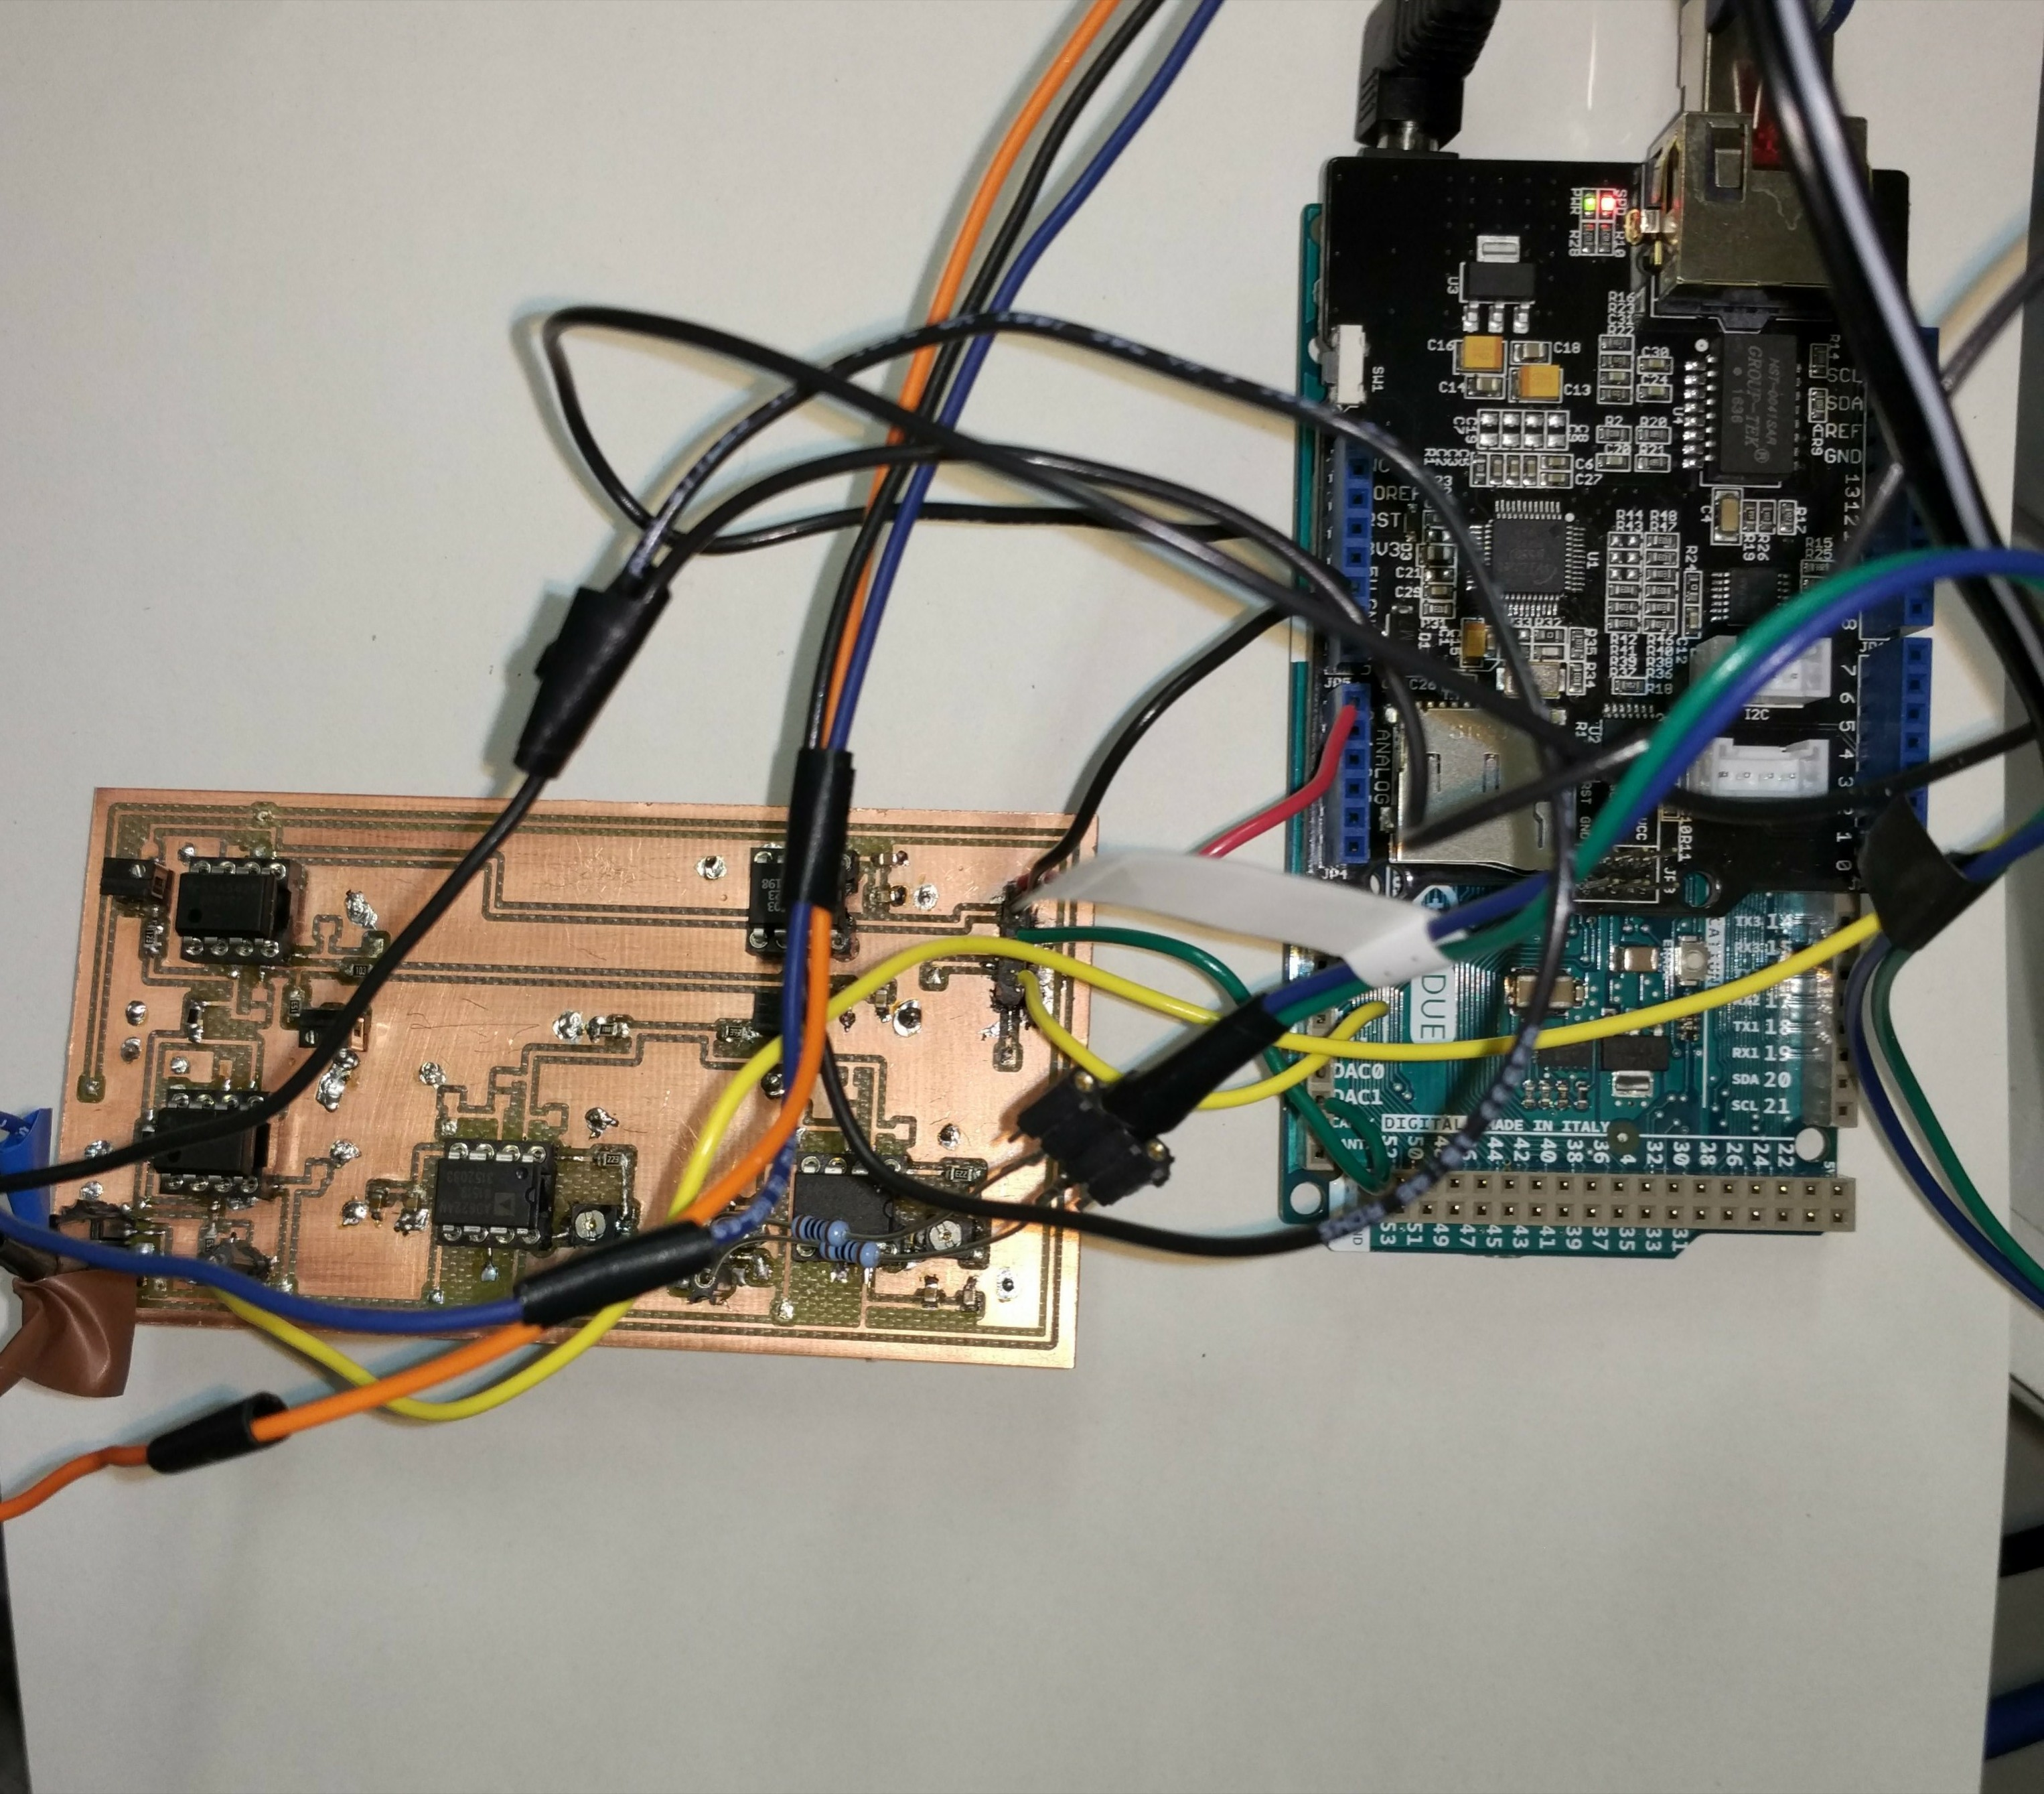
\includegraphics[width = \textwidth]{boardwitharduino.jpg}
        \caption{Board connected to Arduino}
        \label{fig6}
      \end{figure}
      After everything on the board is done it is put into the housing in the
      cabinet.
      \begin{figure}[H]
        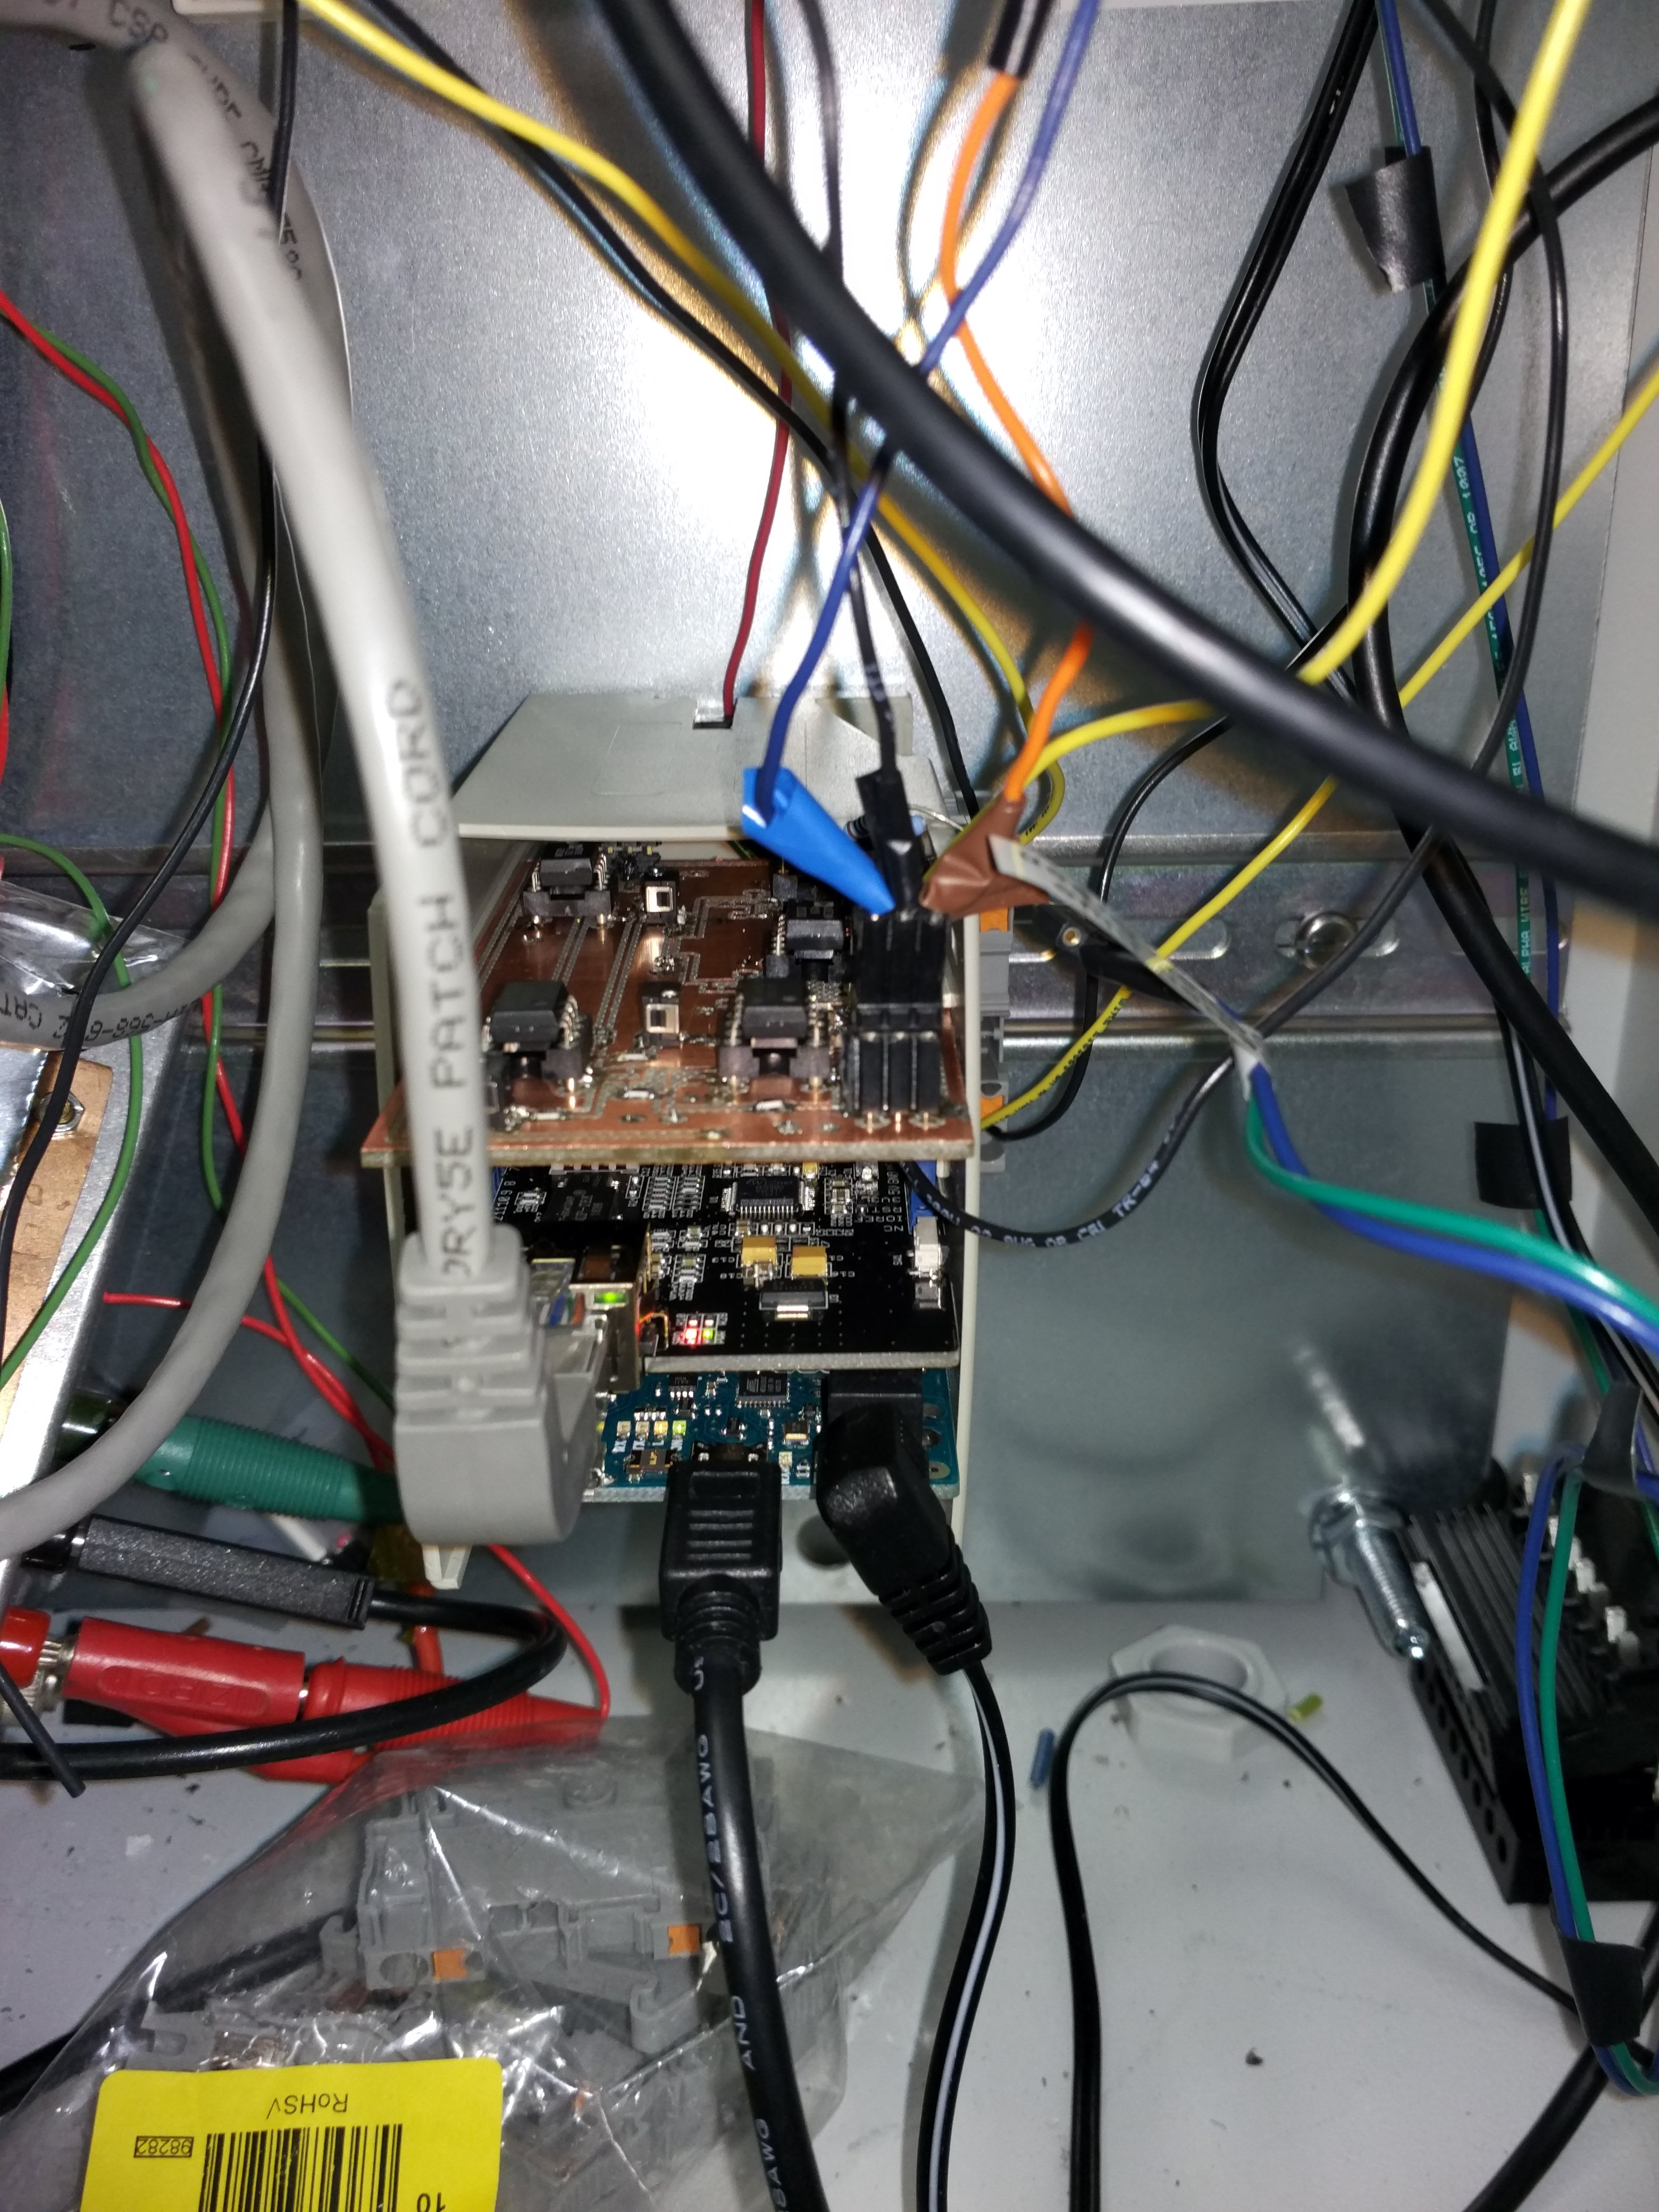
\includegraphics[width = \textwidth]{imschrank.jpg}
        \caption{Board and Arduino in the housing}
        \label{fig7}
      \end{figure}
    \section{Measurements}
      \subsection{Measurements for the heater/cooler shifter circuit}
        I measure the output voltage from the heater and cooler shifter while
        changing the input through the Arduino DAC outputs. The DAC outputs use
        8Bit resolution, so we measure from 0 to 255 Bits.
        \begin{figure}[h]
          \subfigure[]{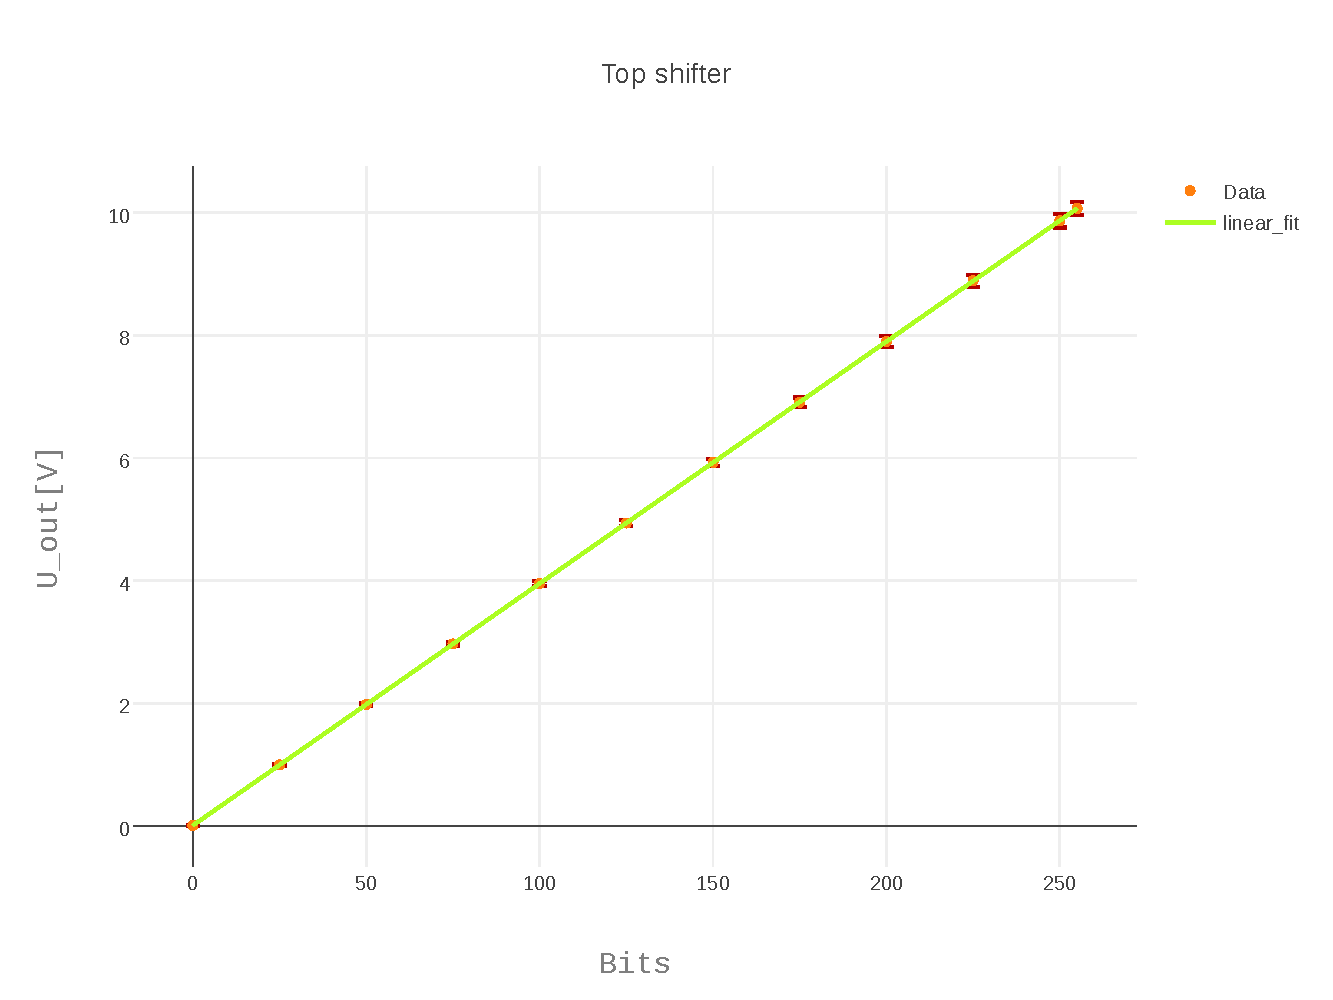
\includegraphics[width = 0.55\textwidth]{./plots/plot_image(1)}}
          \subfigure[]{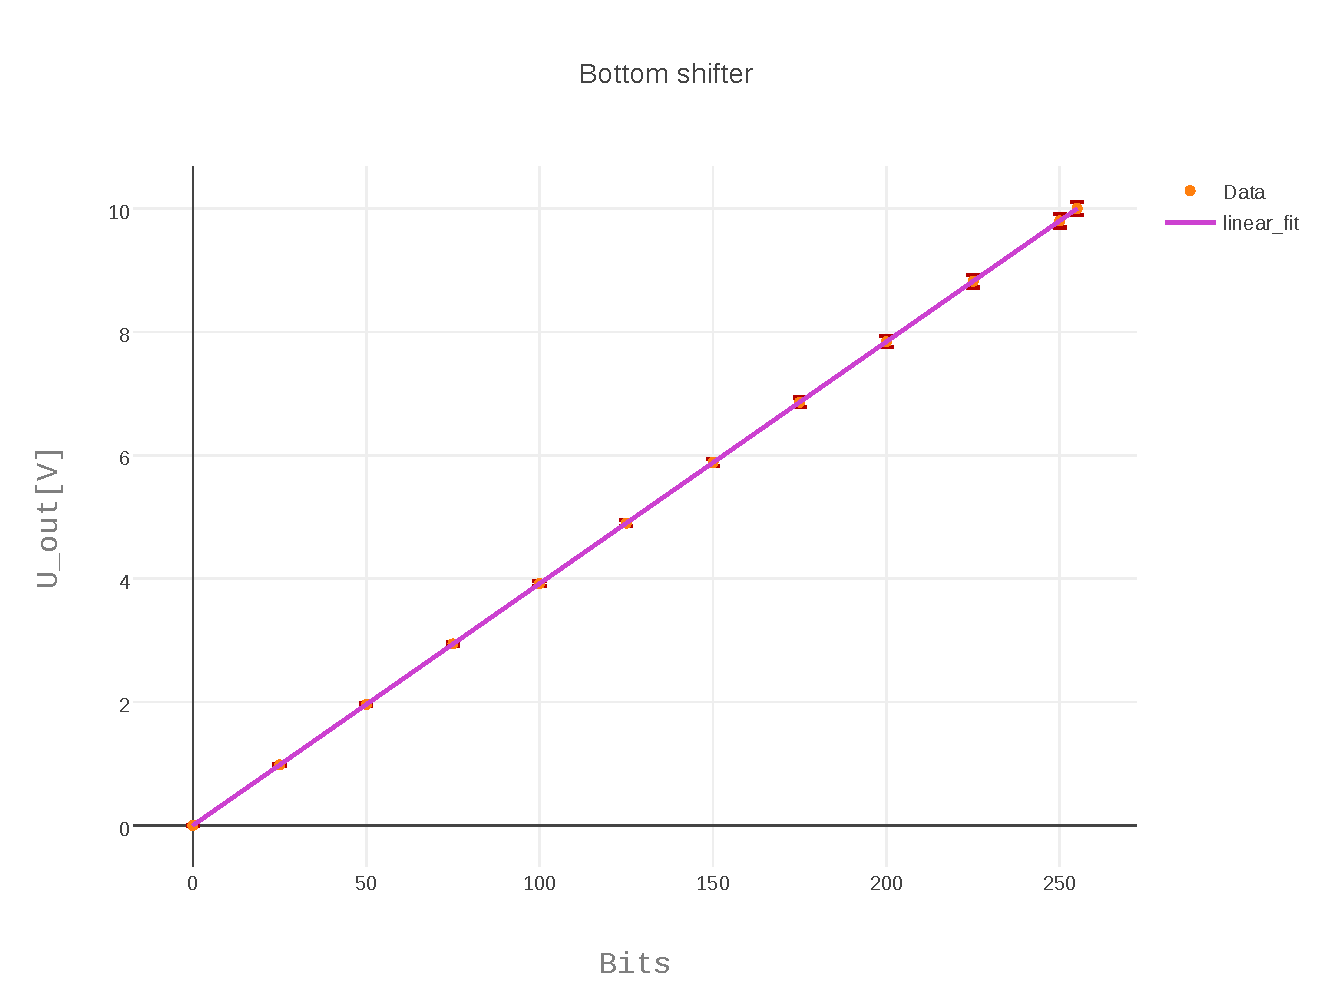
\includegraphics[width = 0.55\textwidth]{./plots/plot_image(2)}}
          \caption{Heater/cooler shifter calibration}
          \label{fig8}
        \end{figure}
        \\It's visible that the components act as expected, i.e. linearity is
        achieved. The minimum out voltages are near enough to 0 and the maximum
        voltages are close enough to 10V.
      \subsection{Measurements of temperature sensor circuit}
        We first measure the voltages (and set them with the variable
        resistances) on the output for the min/max values -1.6V/1.6V and make
        sure that above/below these voltages the output voltage does not change
        anymore. Then we measure the values inbetween.
        \begin{figure}[h]
          \centering
          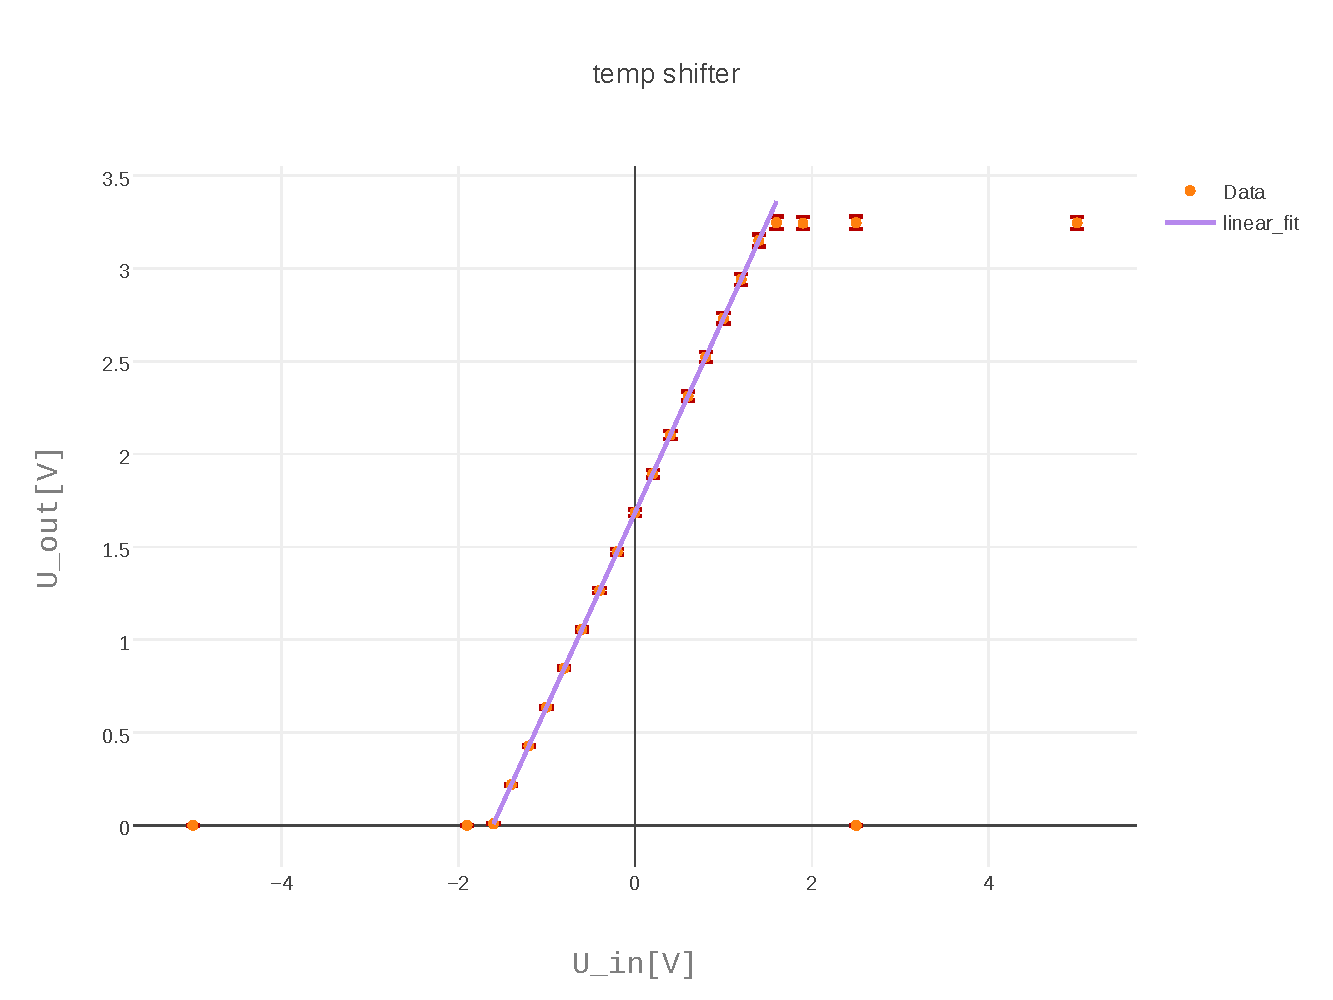
\includegraphics[width = 0.55
          \textwidth]{./plots/plot_image(3)}
          \caption{Response of the temp. shifter}
          \label{fig9}
        \end{figure}
        \\ We see that we have linearity between -1.6V and 1.6V (slight drop
        before 1.6V) and afterwards the desired plateaus.
    \section{The temperature control system}
      \subsection{Controlling the PID} \label{sec:control}
      The temperature value gets read out on a Arduino Due platform. It then
      checks with the temperature reference and calculates control values
      for the heater / cooler with a PID controller, which was realized as a
      software running on the Arduino. This was originally developed by Vanessa
      Scheller.
      \\One of my tasks was to install the Ethernet Shield 2 on the Arduino in
      order for the PID controller to be abled to communicate more easily with
      a computer. The existing possibility to communicate with the Arduino was
      to do it over the usb serial interface of the Arduino which allows to
      read out data and also send data to the Arduino, but requires a computer
      to be connected to the Arduino at all times. The advantage of a network
      interface is that it just needs a connected ethernet cable to the Arduino.
      \\The Ethernet Shield 2 is just connected to the Arduino like any other
      Arduino shield, by just plugging it on top of the Arduino. The Arduino
      acts as a server which communicates with a client program
       running on the tritium-vserver.
      \\The client sends commands directly to the Arduino which get handled
      there in a defined time intervall. The Arduino sends back a response
      including information.
      \\The client program runs in the background and issues the command to
      receive the serial output from the Arduino and stores those directly in
      a file as is, but also creates a THee file with only the time and the
      temperature values.
      \\The client program can be controlled with the
      controller script. Running the script with a
      command line argument makes the client program send the argument as a
      command to the Arduino. The answer from the Arduino is stored in a log
      file and also printed on the console.
      The commands are to be send as follows:
      \\\\
      \textbf{Getting the serial output} \\
      Send the command \textbf{\textit{g}} to receive the serial output. The values
      received are:
      \begin{enumerate}
        \item Measurement number (resets every new running day)
        \item Mean temperature value over 1 minute. (in 10 bit resolution from
          0 to 1023)
        \item Difference of current temperature to set value of temperature
        \item Difference of mean temperature to set value of temperature
        \item Heater set value (in 8 bit resolution from 0 to 255)
        \item Cooler set value (in 8 bit resolution from 0 to 255)
        \item Days running
      \end{enumerate}\hspace{10pt}

      \noindent\textbf{Getting the PID parameters and the temperature set value} \\
      Send the command \textbf{\textit{gpid}} to receive the values $K_P$, $T_N$
      and $T_V$ for both the heater and the cooler as well as the current
      temperature set value (which is titled sollwert). Also get the state of
      the PID (1 for turned on, 0 for turned off).\\

      \noindent\textbf{Setting the PID parameters and setting fixed heater/cooler
      set values} \\
      Send the command \textbf{\textit{xy\#\#\#}}, where \textit{x} is either
      \textit{h} or \textit{c} for heater/cooler and \textit{y} is either
      \textit{p,i,d} for the respective part of the regulator. \textit{y} can
      also be \textit{f} for a fixed value of the heater/cooler set value (this
      turns off the PID control). \#\#\# corresponds to the wanted value (again in
      8 bits from 0 to 255). The Arduino programm checks whether the value is
      in bounds.\\

      \noindent\textbf{Setting the temperature reference}\\
      Send the command \textbf{\textit{so\#\#\#}} to set the temperature
      reference to the value \#\#\# (in 10 bits).\\

      \noindent\textbf{Turning PID off and back on}\\
      Send the command \textbf{\textit{pidon / pidoff}} to turn the PID on or off.
      If the PID is turned off it will use the fixed values for the set values of
      the heater and cooler (default is zero for both).\\

      \noindent The calibration for the temperature values of the sensor is shown
      below.
      \begin{figure}[h]
        \centering
        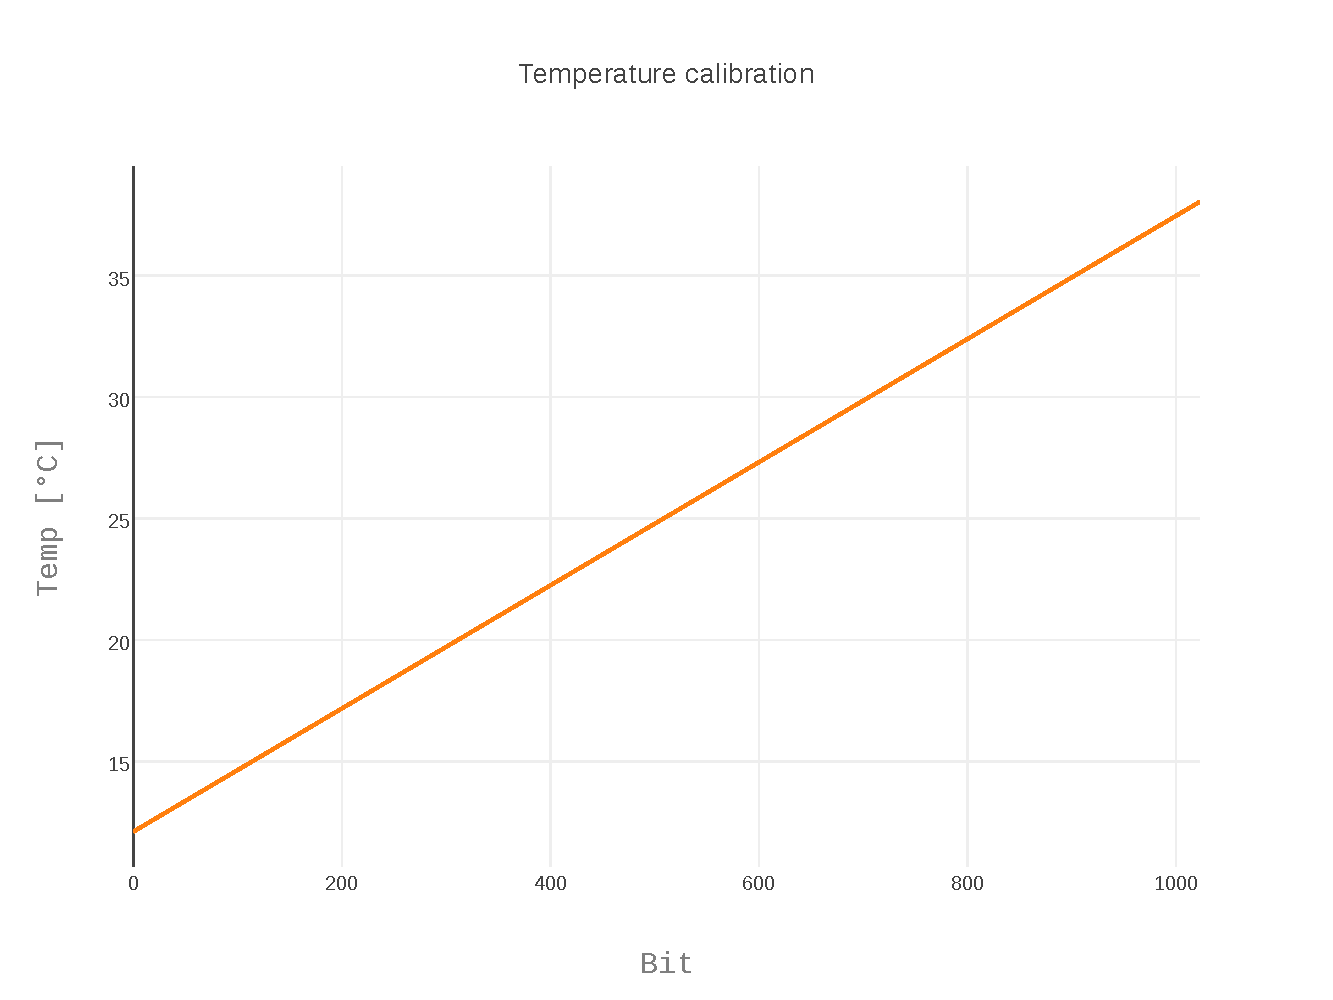
\includegraphics[width = 0.65\textwidth]{./plots/plot_image(4)}
        \caption{Calibration of temperature sensor}
        \label{fig10}
      \end{figure}
      \\
    \subsection{Testing the temperature control system}
      The board is now connected to the Arduino, the temperature sensor and the
      heater/cooler. \\
      Now I measure for a constant temperature reference the temperature with
      already existing sensors (i.e. top window, top door and the PID temperature
      sensor).
      \subsubsection{Holding the temperature constant}
        We want to see now, how well the temperature stabilization works for
        keeping the temperature constant over the day (18.02.2017). We get the
        data for one day from the THee-Files located in the tritium-drive (the
        pid-client program also produces Thee-files there). See
        Figure~\ref{fig11} (a-c) for the temperatures.
        Also a histogram of the data at the PID-sensor is plotted in
        Figure~\ref{fig11} (d).
        \begin{figure}[h!]
          \hspace{-40pt}
          \subfigure[]{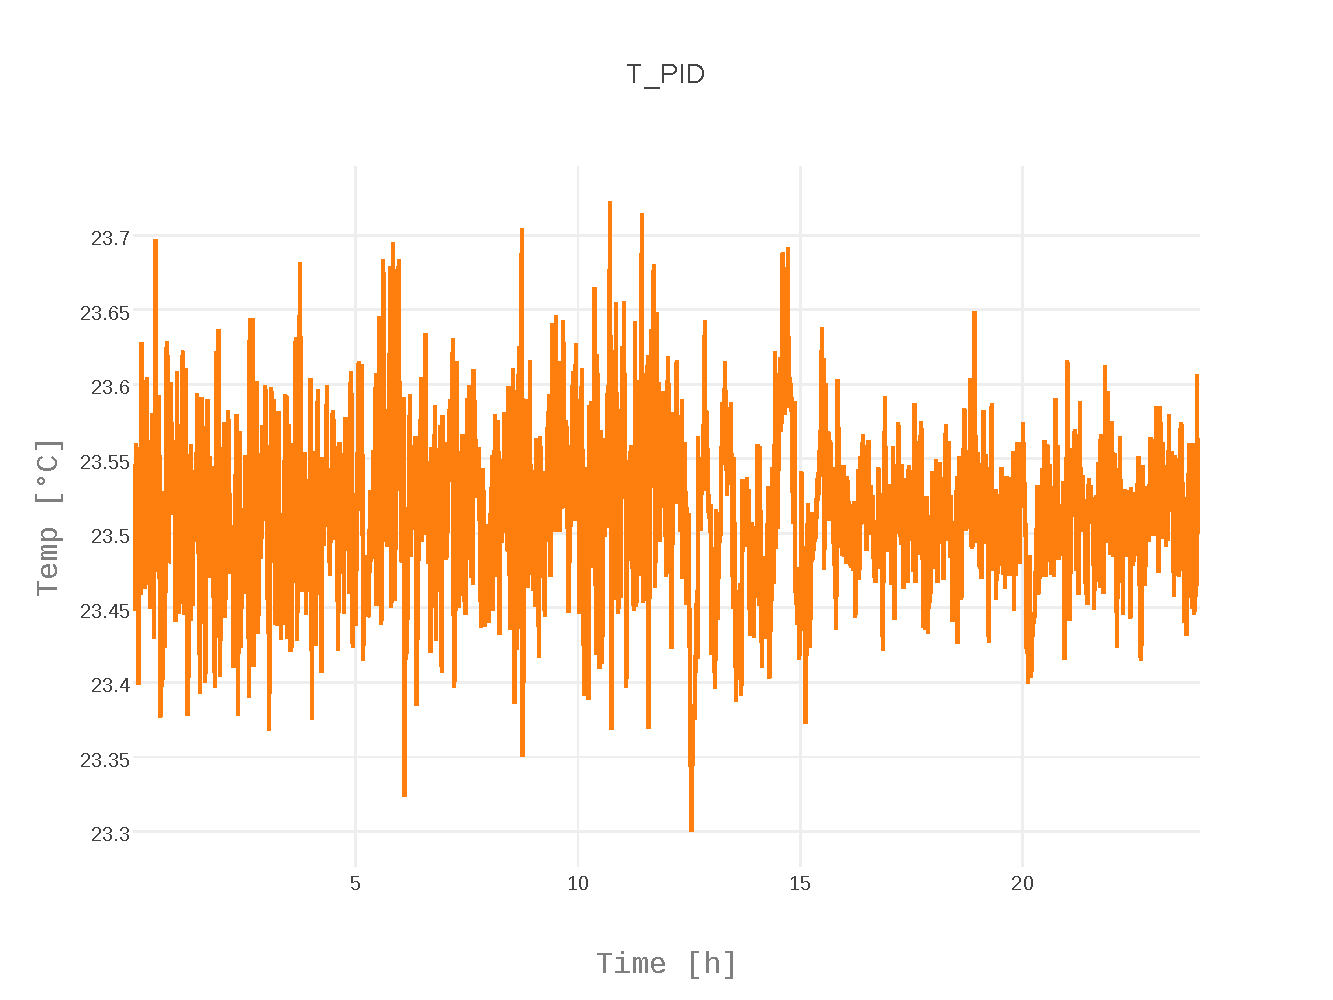
\includegraphics[width = 0.65\textwidth]{./plots/plot_image(5)}}
          \hspace{-20pt}
          \subfigure[]{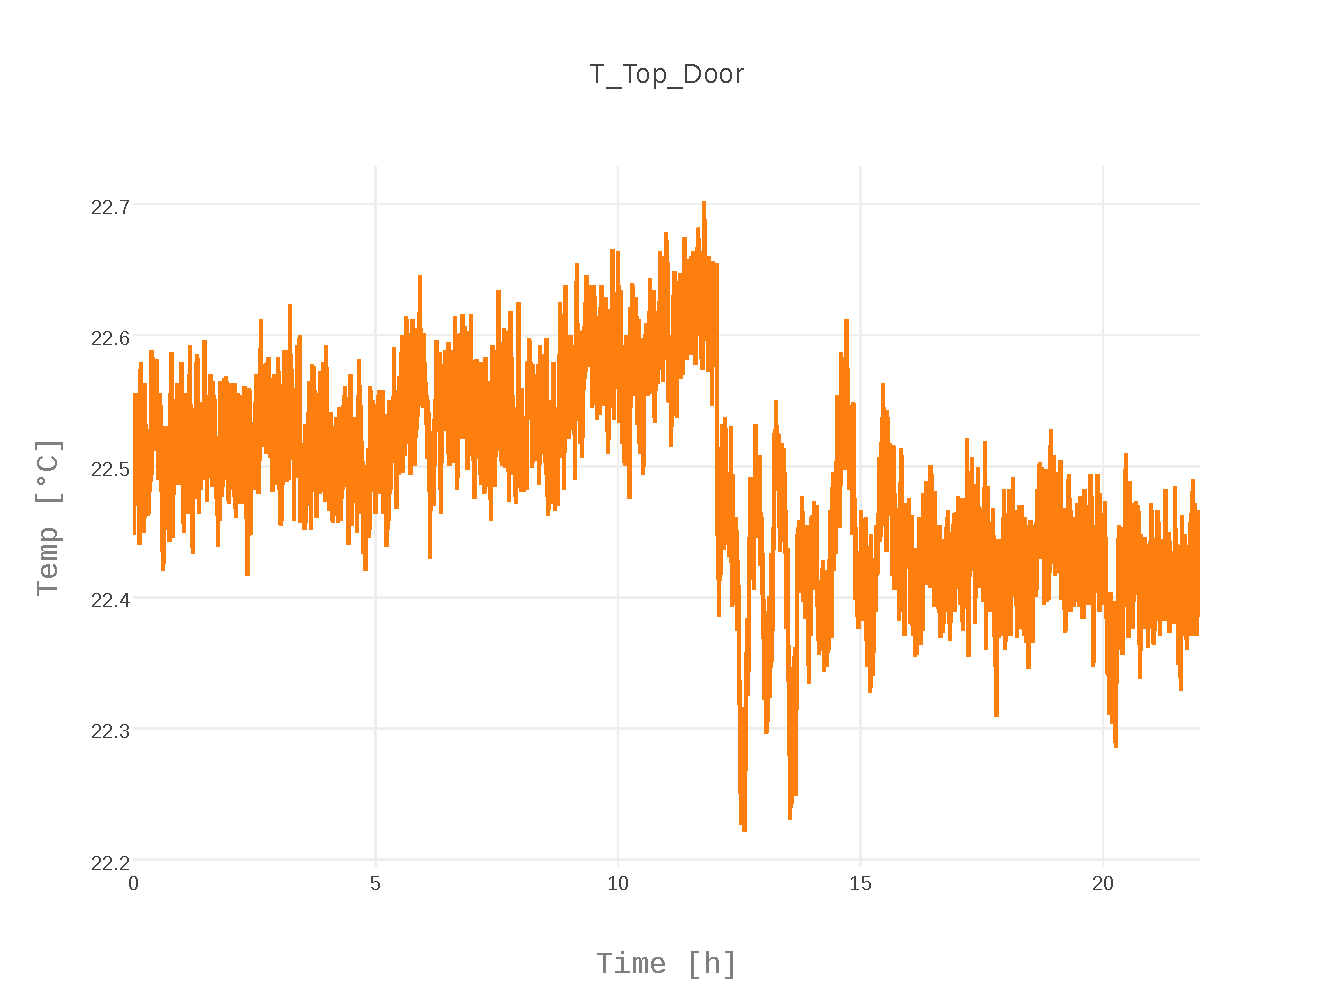
\includegraphics[width = 0.65\textwidth]{./plots/plot_image(6)}}
          \subfigure[]{\hspace{-40pt}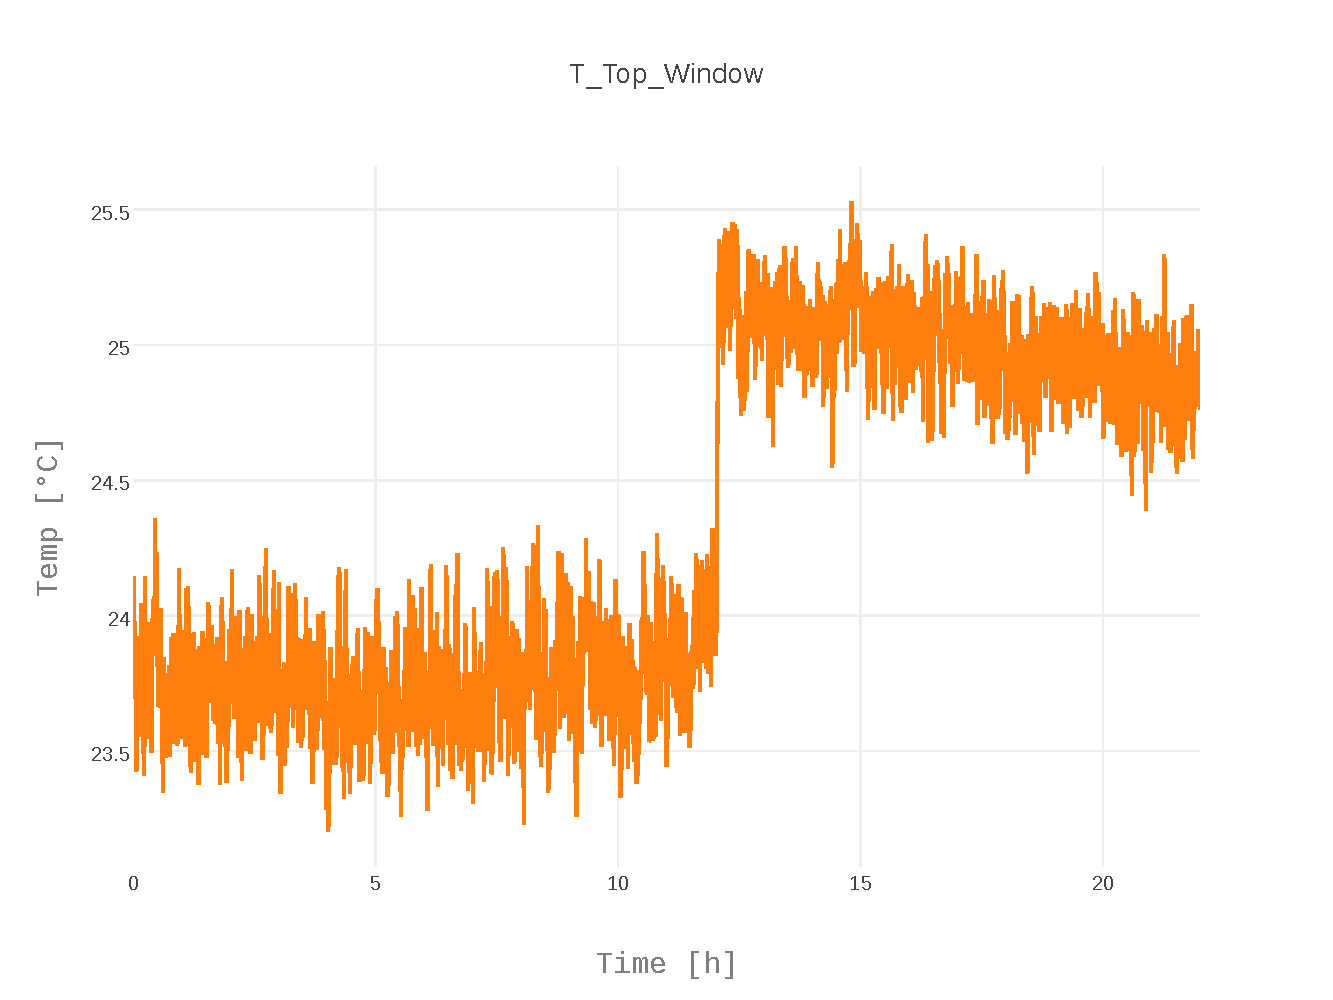
\includegraphics[width = 0.65\textwidth]{./plots/plot_image(7)}}
          \subfigure[]{\hspace{-20pt}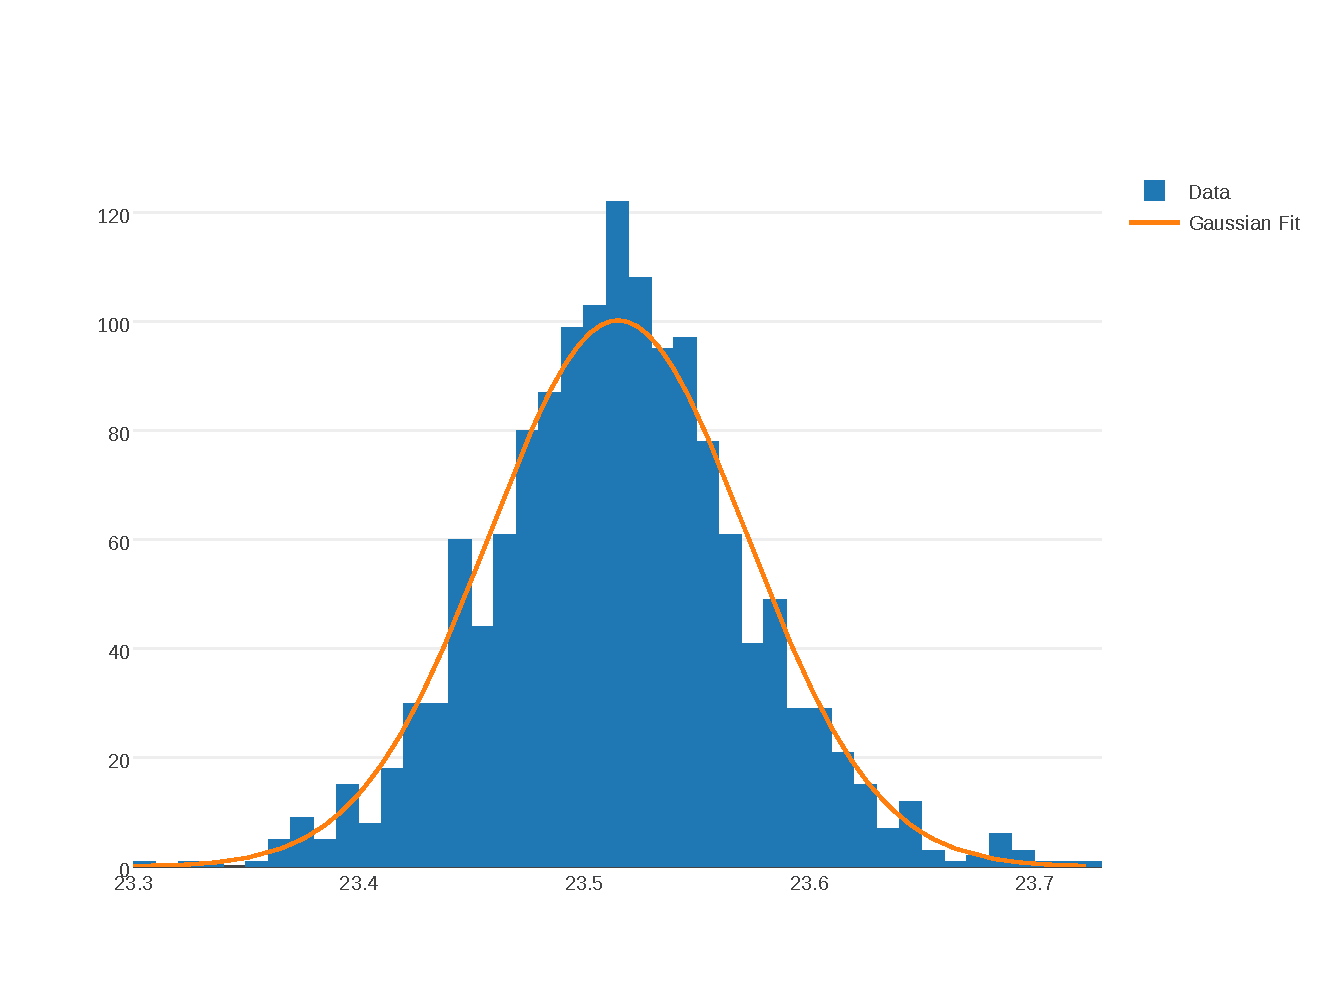
\includegraphics[width = 0.65\textwidth]{./plots/plot_image(8)}}
          \caption{Temperature stabilization over one day with temp. from
          sensors T\_PID, T\_Top\_Door, T\_Top\_Window.}
          \label{fig11}
        \end{figure} \\
        The mean of the histogram is at $\mu = 23.515\,\text{°C}$ and the standard
        deviation at $\sigma = 0.057\,\text{K}$. \\
        We see that for the sensor the PID uses to regulate to we have a good
        nearly constant temperature (fluctuations $\sim 0.5\,\text{K}$ and
        $\sigma = 0.057\,\text{K}$). The other two sensor show a fast rise
        (window) and a fall(door) in temperature at around 12 o'clock. I can now
        look at the cooler/heater values and see that the cooler was shut off up
        until nearly 12 o'clock and then turned on (probably due to rise in
        outside temperature), while the heater value decreased. \\
        The heater is located closer to the window and the cooler closer to the
        door.
        The rise in outside temperature could be due to sun coming in the
        windows thus raising the temperature there fast. The drop at the door
        should then be due to the cooler being turned on.
      \newpage
      \subsubsection{Change in temperature reference}
      To see how the system reacts to rapid changes in temperature it is much
      easier to look at a change in the reference temperature. For this we
      change the value of the reference temperature from 450 Bits ($\sim 23.5
      \,\text{°C}$) to 500 Bits ($\sim 24.8 \,\text{°C}$). \\
      Again we look at the temperature values from the 3 sensors.
      \begin{figure}[h!]
        \hspace{-40pt}
        \subfigure[]{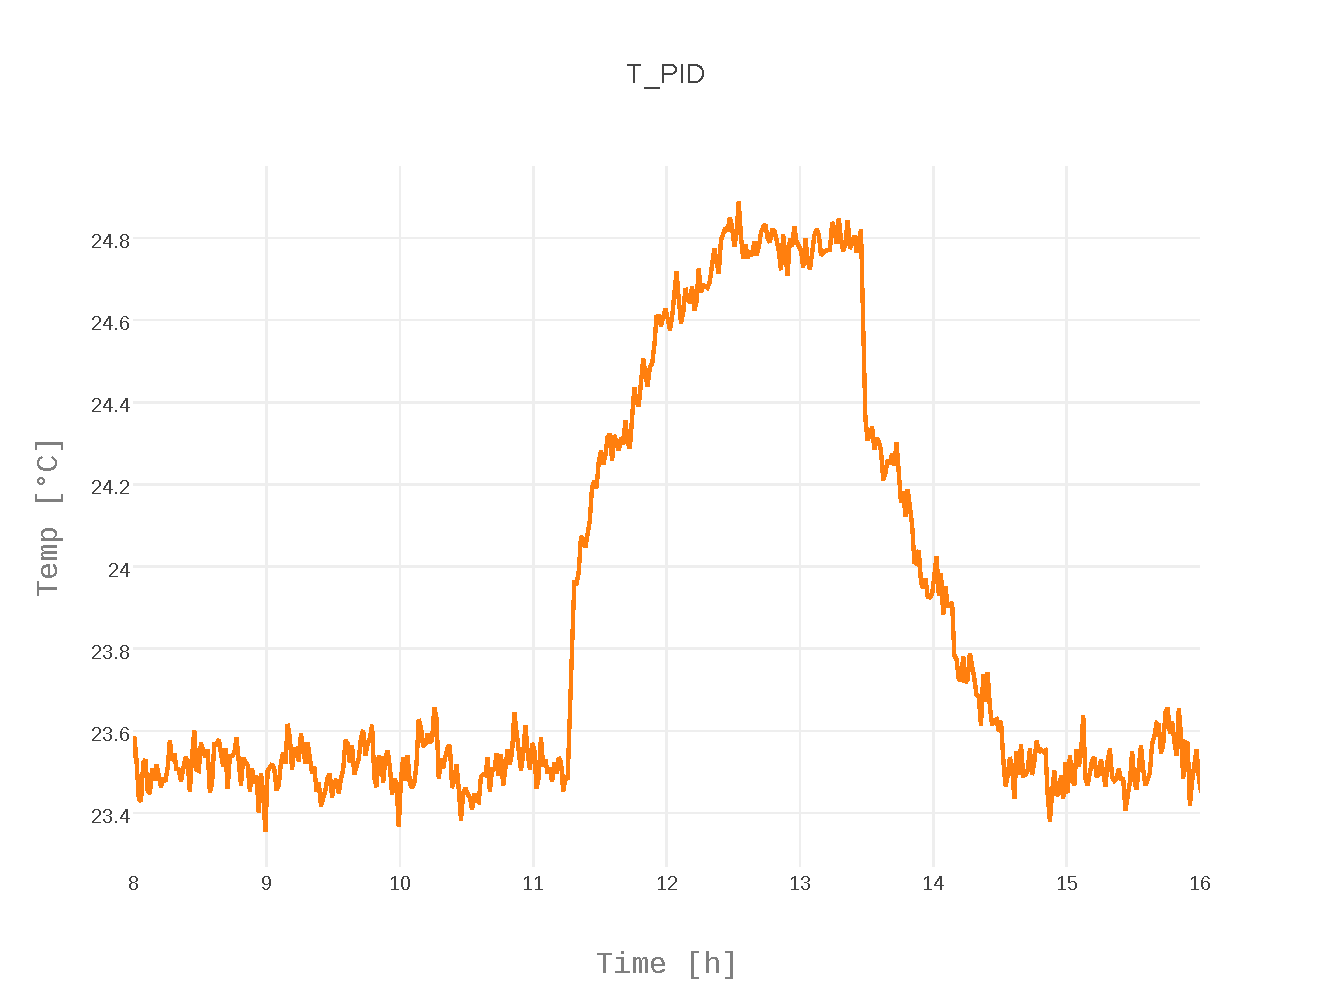
\includegraphics[width = 0.65\textwidth]{./plots/plot_image(9)}}
        \hspace{-20pt}
        \subfigure[]{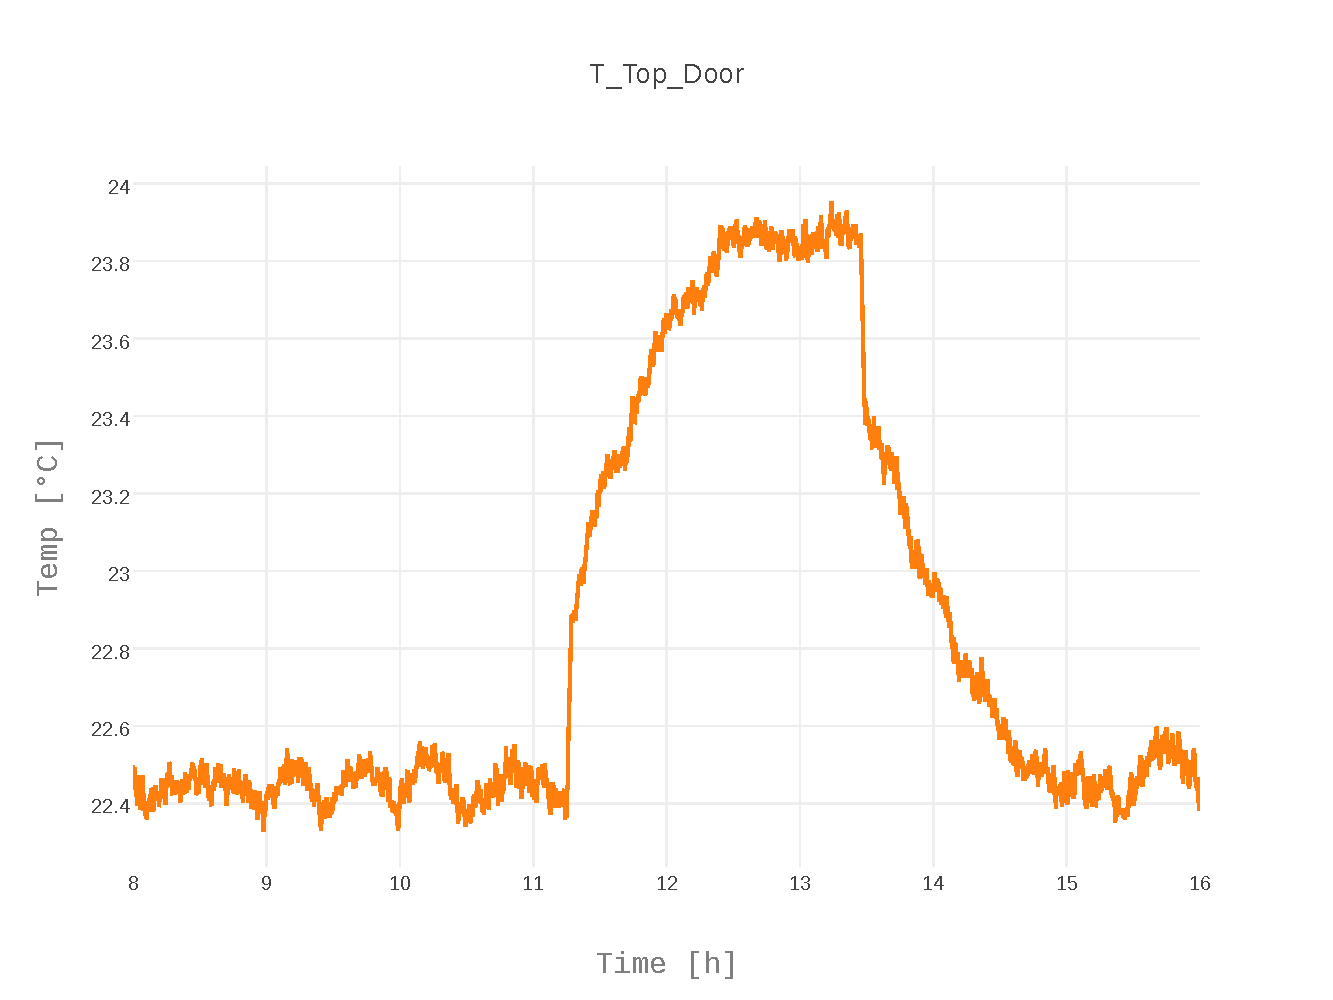
\includegraphics[width = 0.65\textwidth]{./plots/plot_image(10)}}
        \subfigure[]{\hspace{3cm}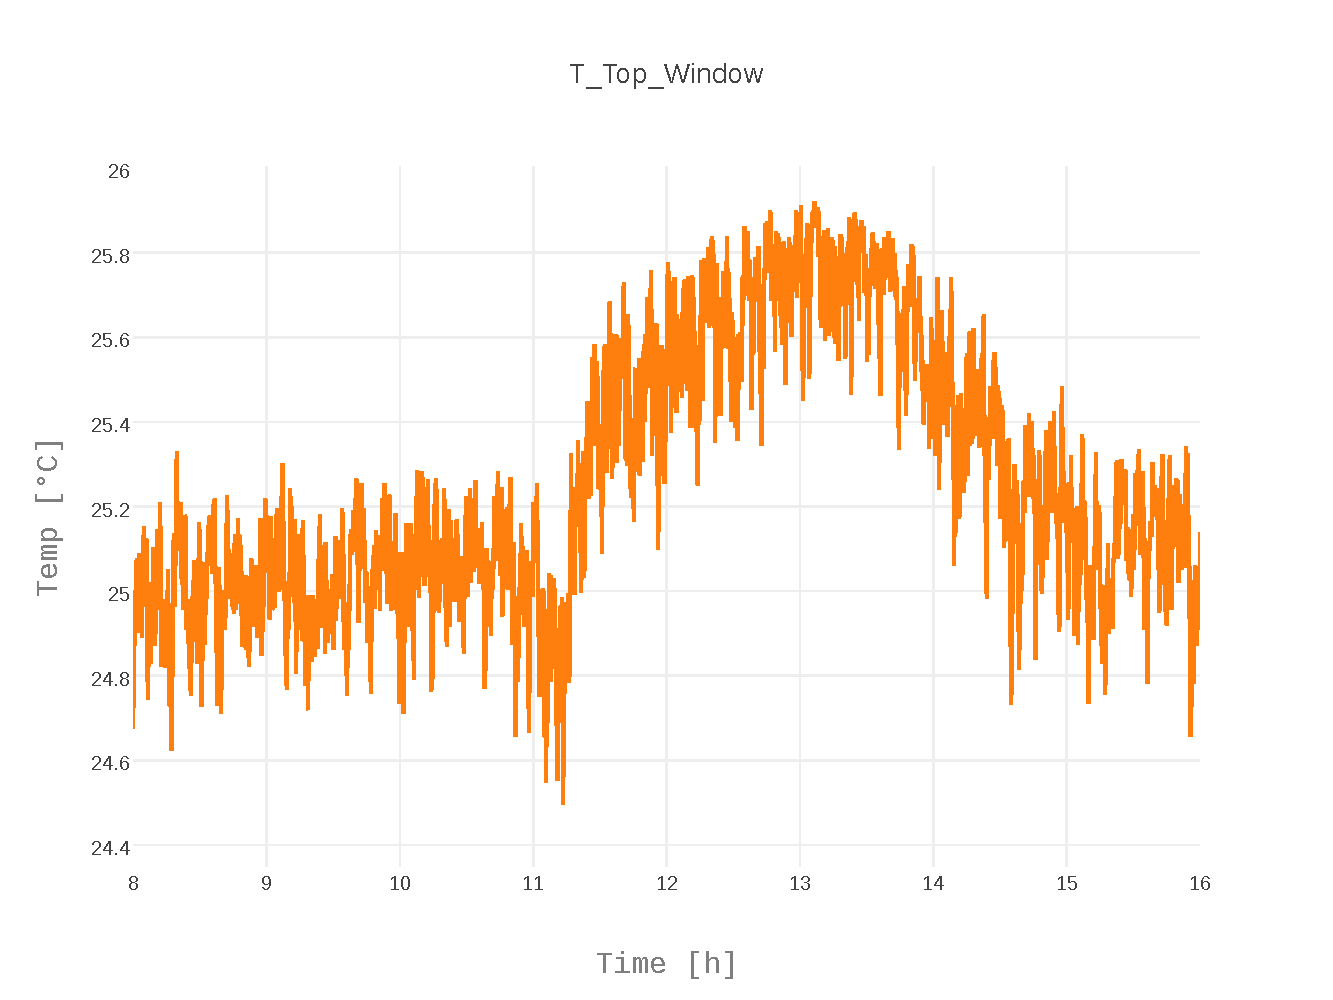
\includegraphics[width = 0.65\textwidth]{./plots/plot_image(11)}}
        \caption{Respose to change in intemperature reference}
        \label{fig12}
      \end{figure} \\
      It's visible that the temperatures at the door and at the PID sensor react
      very similarly, the temperature at the window seems to react a little
      slower.\\
      I can now compute the time constant of the system with the following fit:
      \begin{equation*}
        f(t) = B + A(1-e^{-t/\tau})
      \end{equation*}
      for the upwards slope and
      \begin{equation*}
        f(t) = B + A e^{-t/\tau}
      \end{equation*}
      for the downwards slope. \\
      For the fit to work we need errors for the temperature values. For this
      we assume a constant error of 0.1 °C. The bounds are set to the time the
      temperature reference was set.
      \begin{figure}[h!]
        \centering
        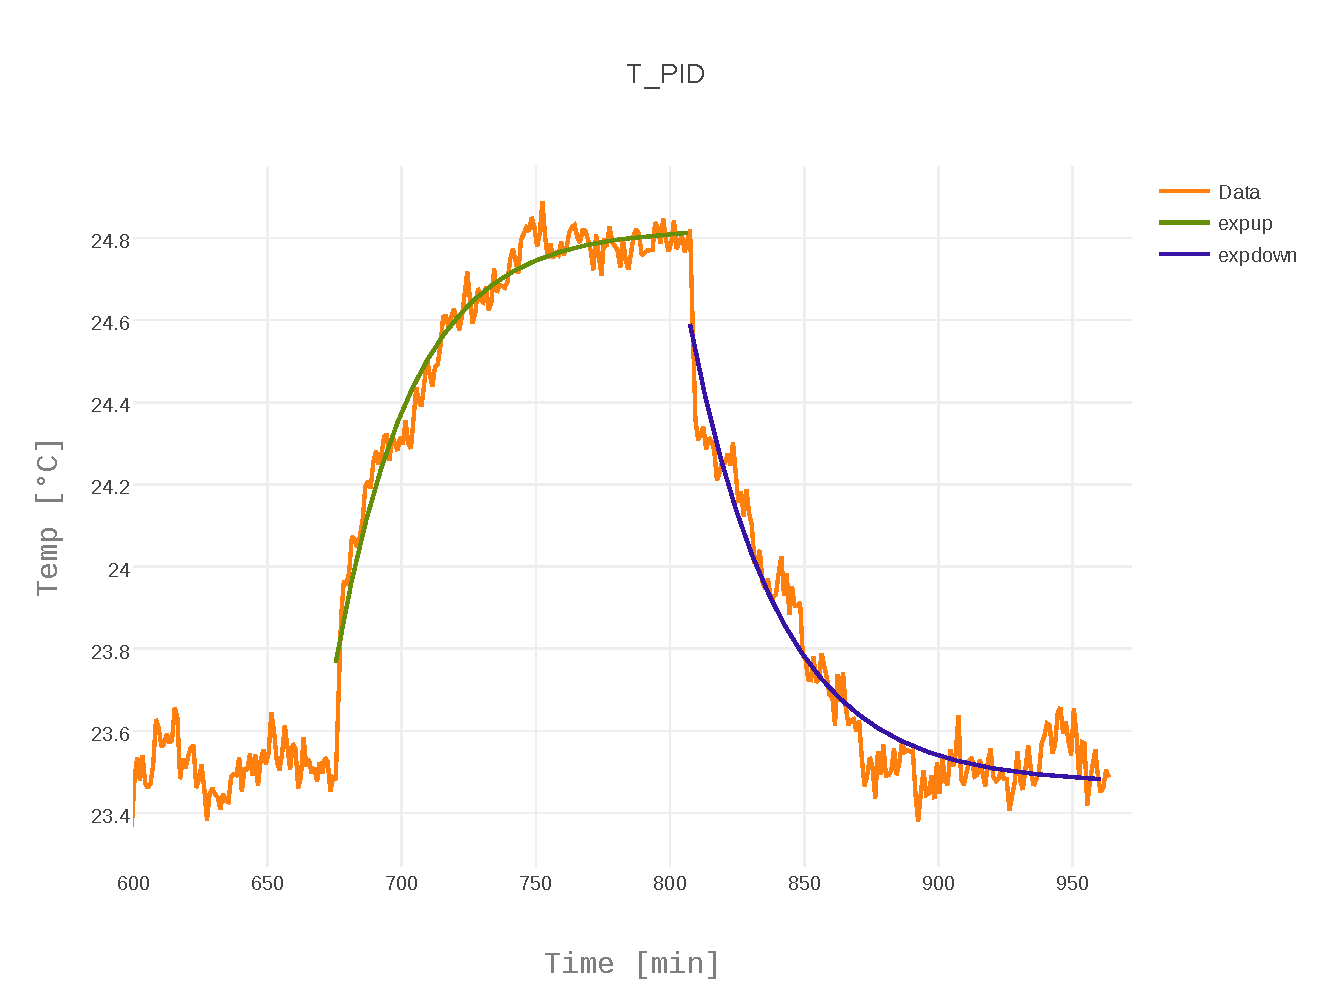
\includegraphics[width = \textwidth]{./plots/plot_image(12)}
        \caption{Response of the PID-controller for a change of 50 bits in
        temperature}
        \label{fig13}
      \end{figure}\\
      The time constants are:
      $$\tau_{\text{up}} = (28.6 \pm 2.3) \,\text{min}, \;\;\; \tau_{\text{down}} =
      (33.1 \pm 2.4)\,\text{min}$$
      It is also visible that the temperature does not overshoot and does not
      strongly oscillate. \\\\
      I do another measurement to confirm the behaviour. This one is done at
      night (Temperature to 500 Bits at 19:11 and back to 450 Bits at 22:45)
      (see Figure~\ref{fig14} ). \\ I also repeat the fitting procedure
      (Figure~\ref{fig15} ). We get a similar value for the upwards slope. The
      downwards slope is slightly faster than before, which might be cause by
      lower outside temperature. We see here that some time after the
      temperature reaches the lower value again it starts to oscillate heavier.
      This is also visible for the Door temperature, which we can also fit
      (Figure~\ref{fig16} ). \\
      Here we get
      $$\tau_{\text{up}} = (32.5 \pm 2.0)\,\text{min}, \;\;\; \tau_{\text{down}} =
      (25.4 \pm 1.5) \,\text{min}$$
      for the PID sensor and
      $$\tau_{\text{up}} = (34.7 \pm 2.0) \,\text{min}, \;\;\;
      \tau_{\text{down}} = (32.7 \pm 1.6) \,\text{min}$$
      for the door sensor.
      \begin{figure}[H]
        \hspace{-40pt}
        \subfigure[]{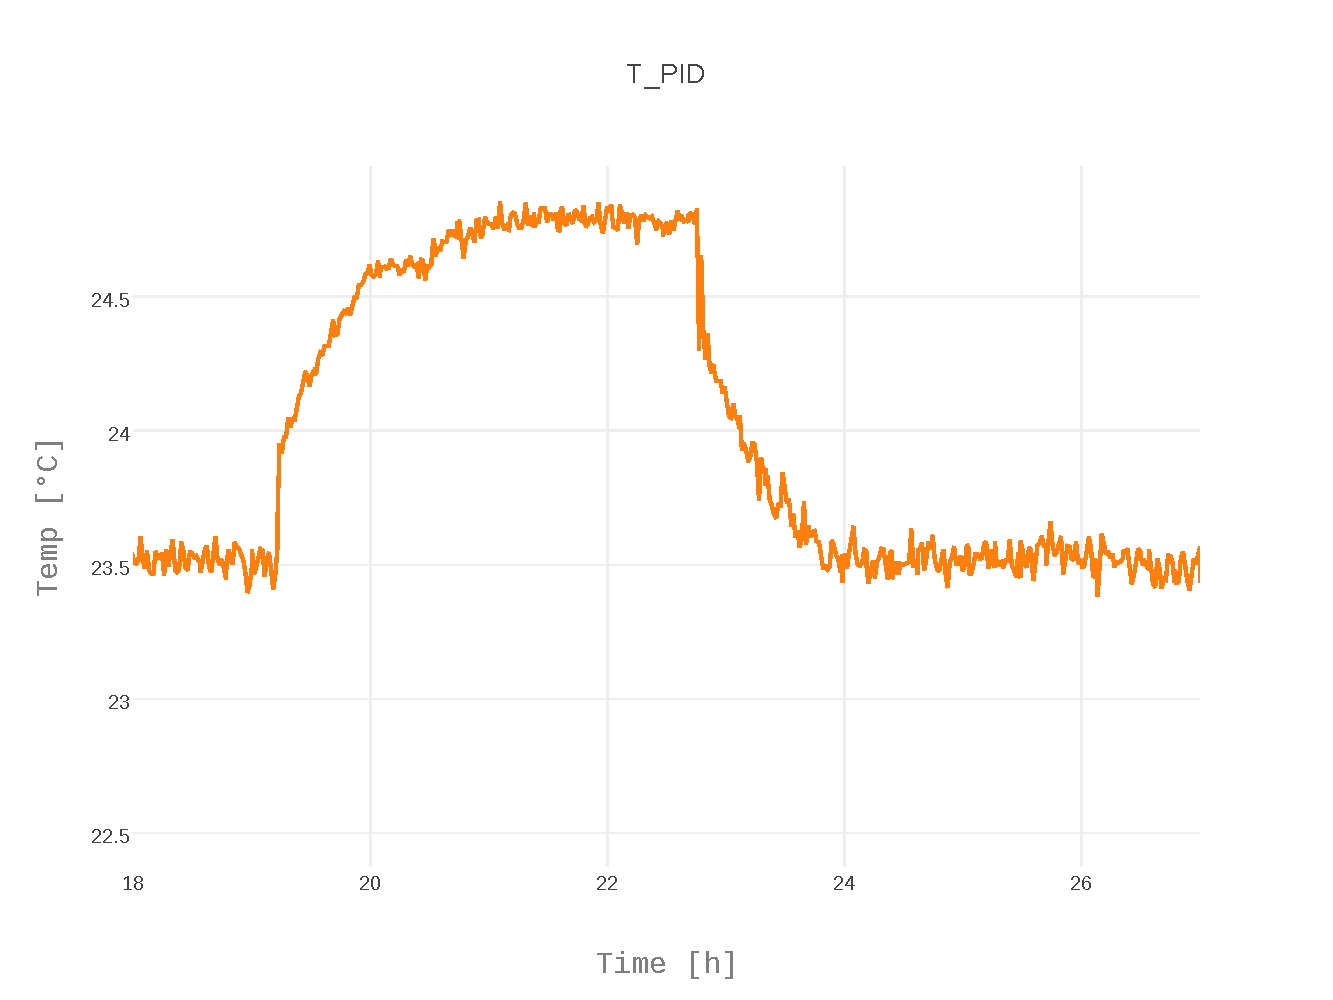
\includegraphics[width = 0.65\textwidth]{./plots/plot_image(13)}}
        \hspace{-20pt}
        \subfigure[]{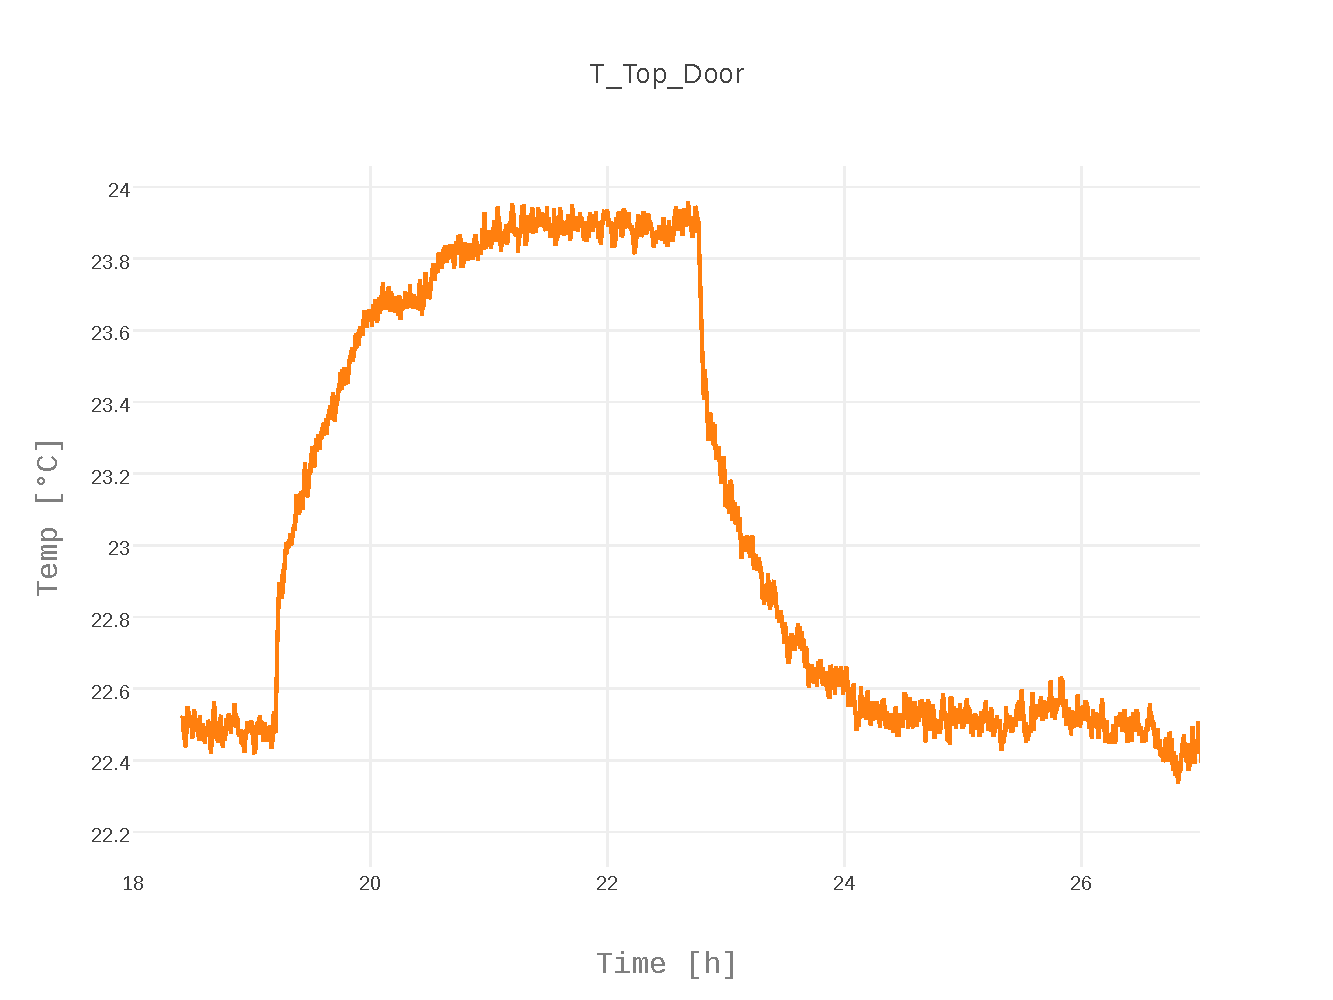
\includegraphics[width = 0.65\textwidth]{./plots/plot_image(14)}}
        \subfigure[]{\hspace{3cm}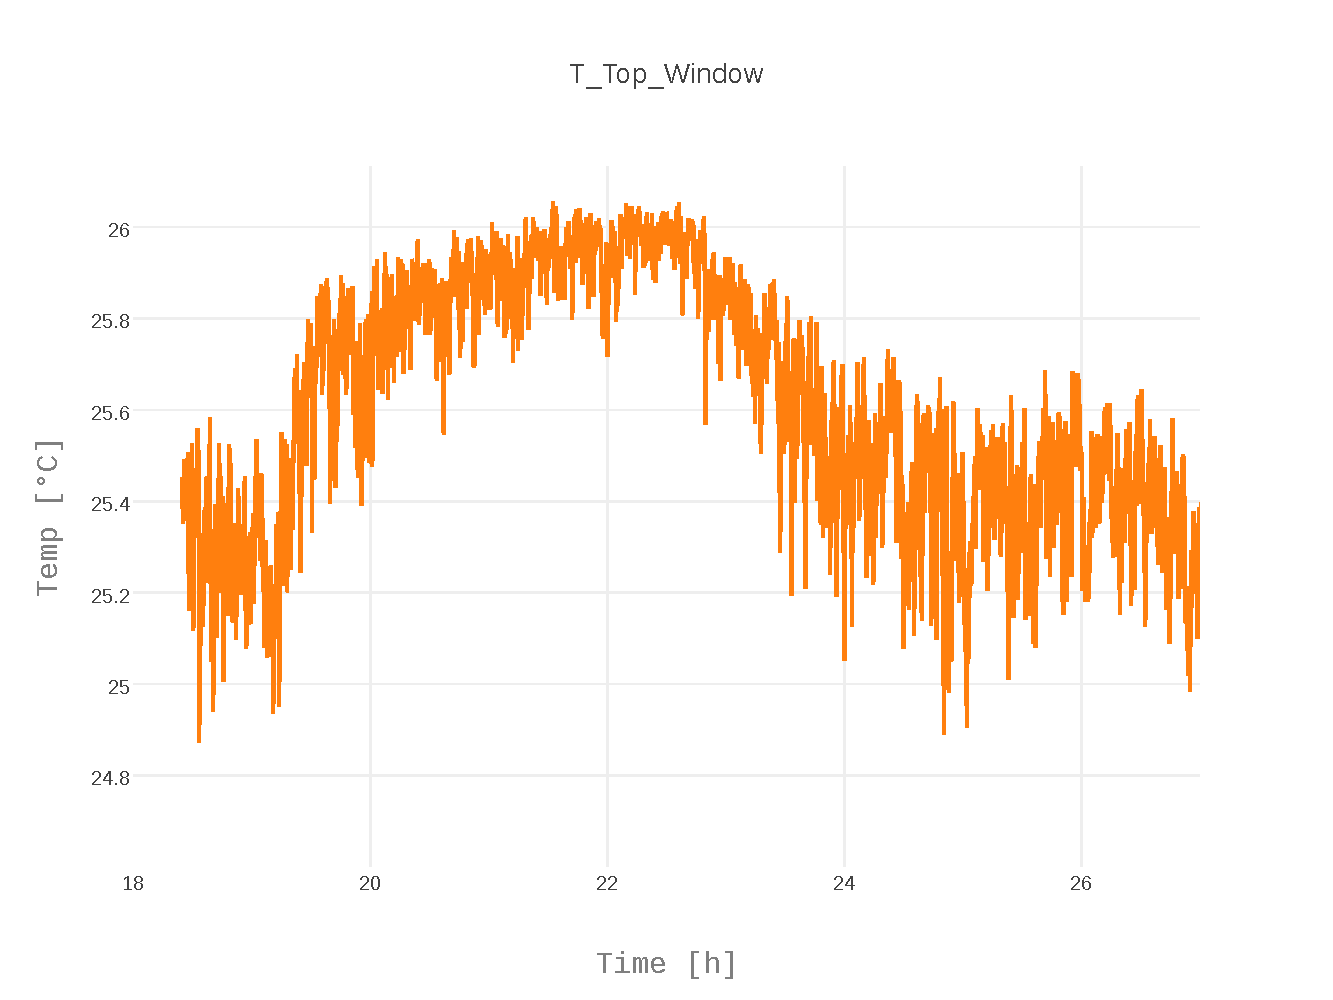
\includegraphics[width = 0.65\textwidth]{./plots/plot_image(15)}}
        \caption{Response to change in intemperature reference}
        \label{fig14}
      \end{figure}
      \begin{figure}[h!]
        \centering
        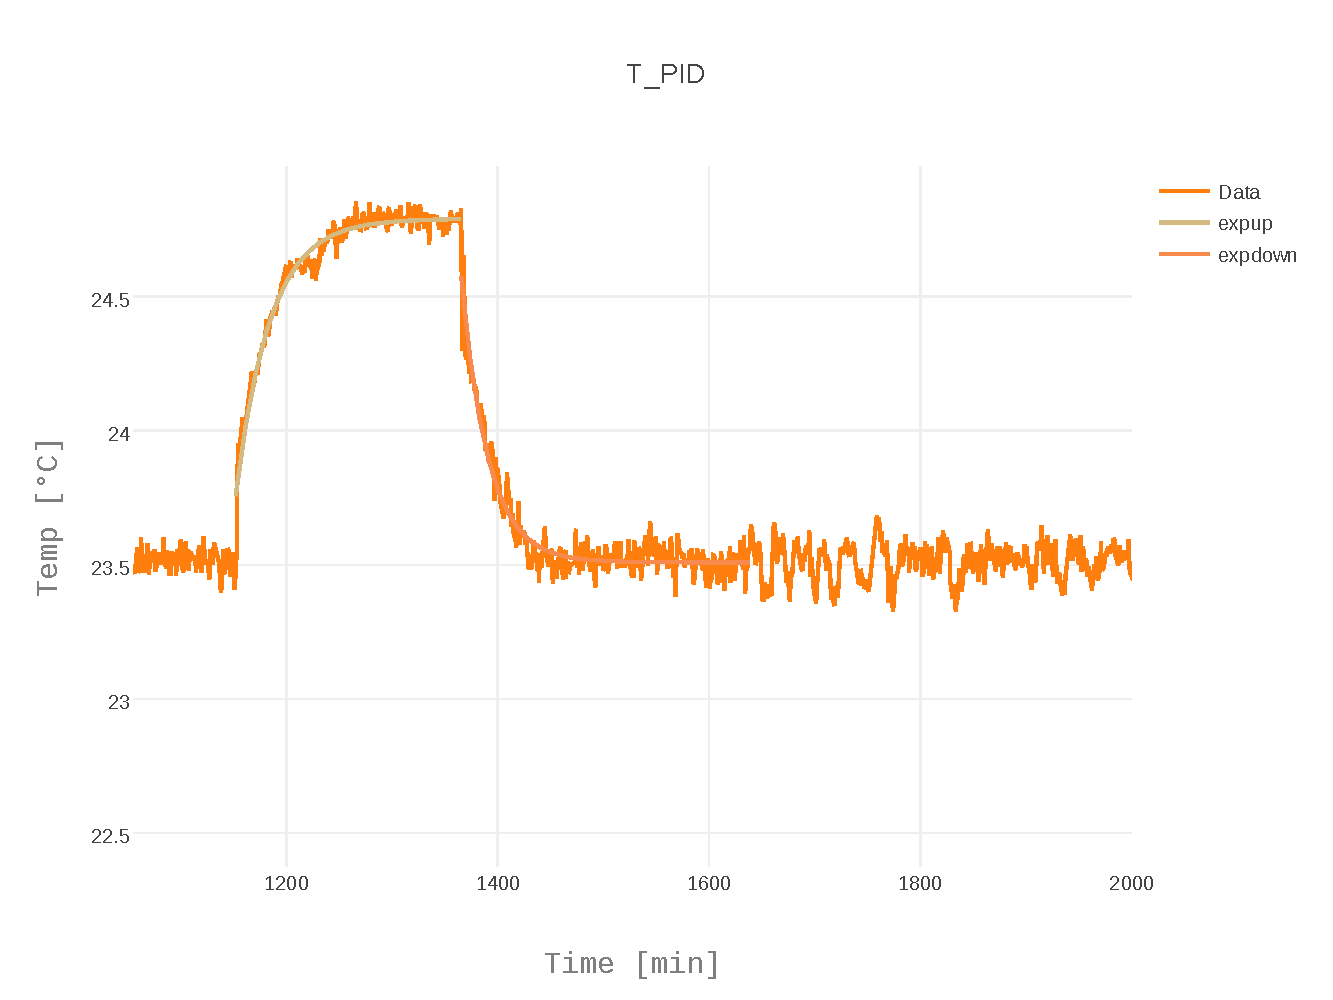
\includegraphics[width = \textwidth]{./plots/plot_image(16)}
        \caption{Step response of PID on PID temp. sensor}
        \label{fig15}
      \end{figure}
      \begin{figure}[h!]
        \centering
        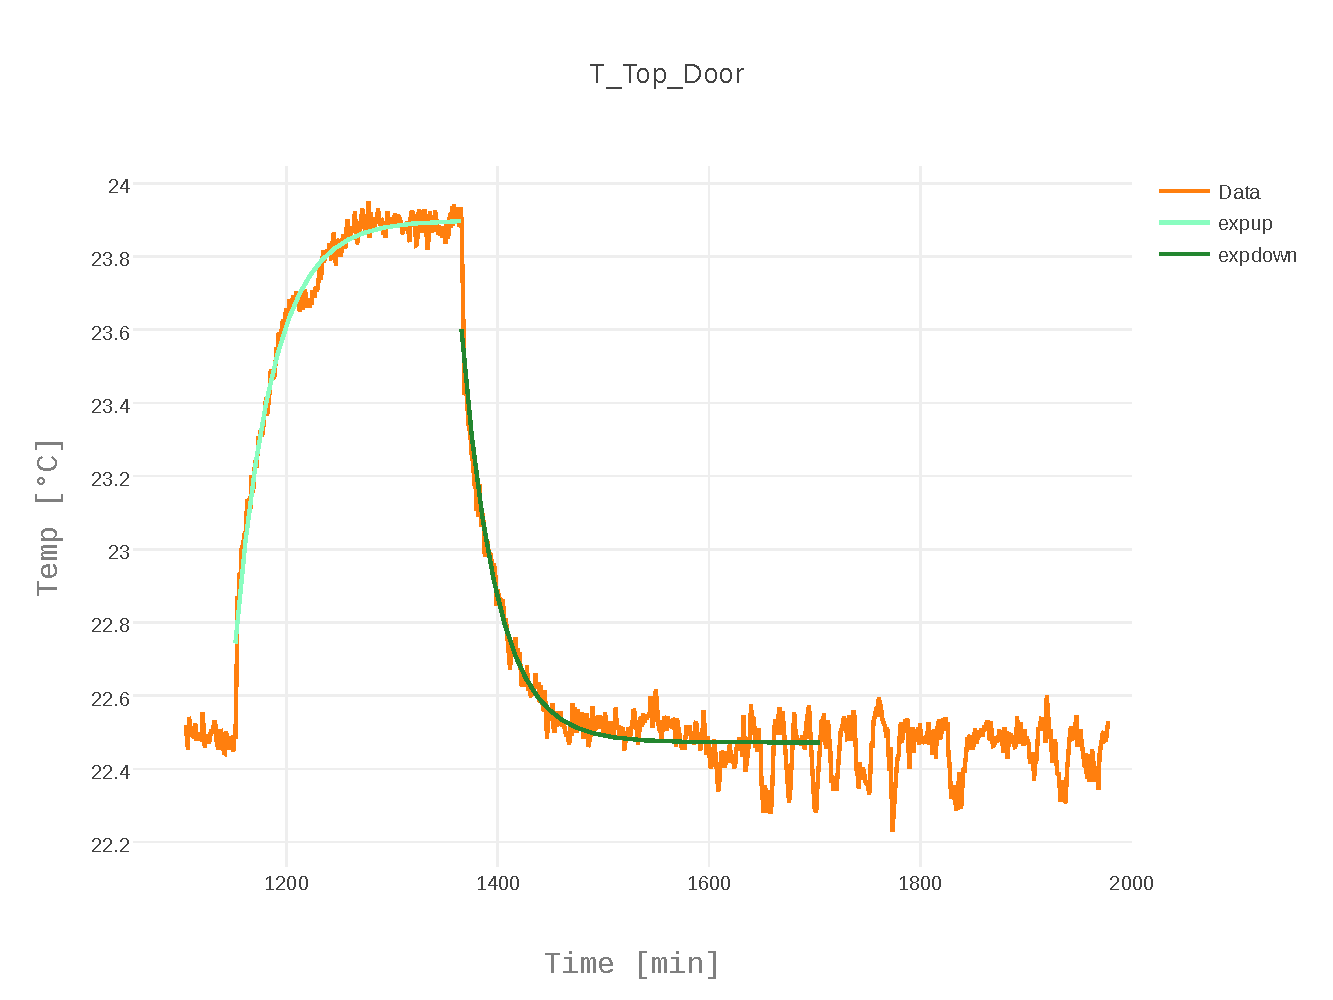
\includegraphics[width = \textwidth]{./plots/plot_image(17)}
        \caption{Step response on Top\_Door temperature sensor}
        \label{fig16}
      \end{figure}
      \clearpage
      \subsubsection{Turning the lights on}
      At 11 o'clock I turn the lights on in the control room. The reaction at
      the different sensors is shown below (Figure~\ref{fig17} ), also the set
      values of the heater/cooler are shown (Figure~\ref{fig18} ).
      \begin{figure}[h!]
        \hspace{-40pt}
        \subfigure[]{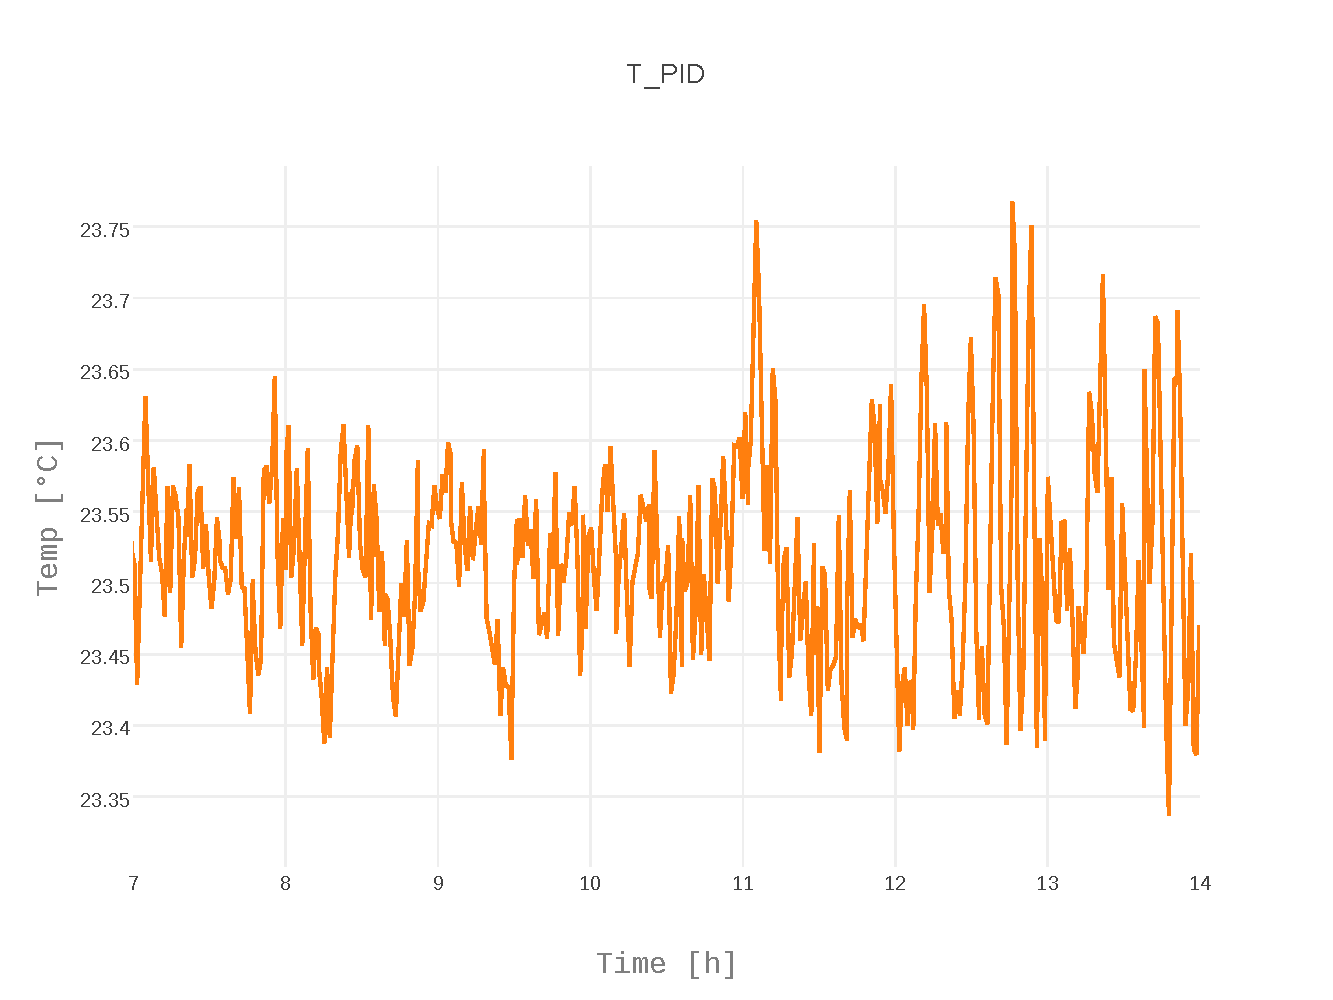
\includegraphics[width = 0.65\textwidth]{./plots/plot_image(18)}}
        \hspace{-20pt}
        \subfigure[]{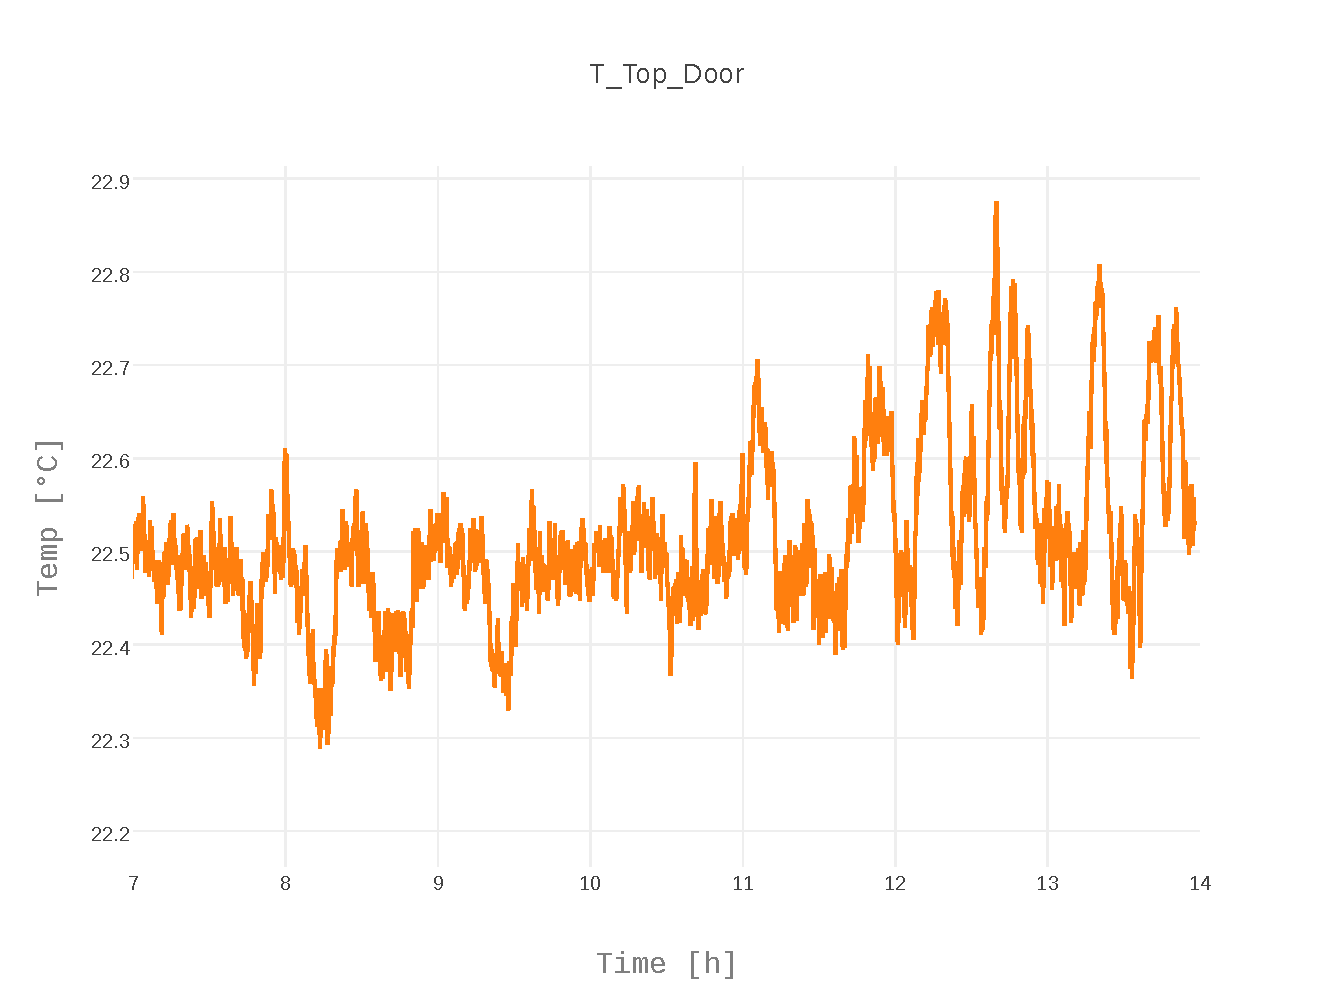
\includegraphics[width = 0.65\textwidth]{./plots/plot_image(19)}}
        \subfigure[]{\hspace{3cm}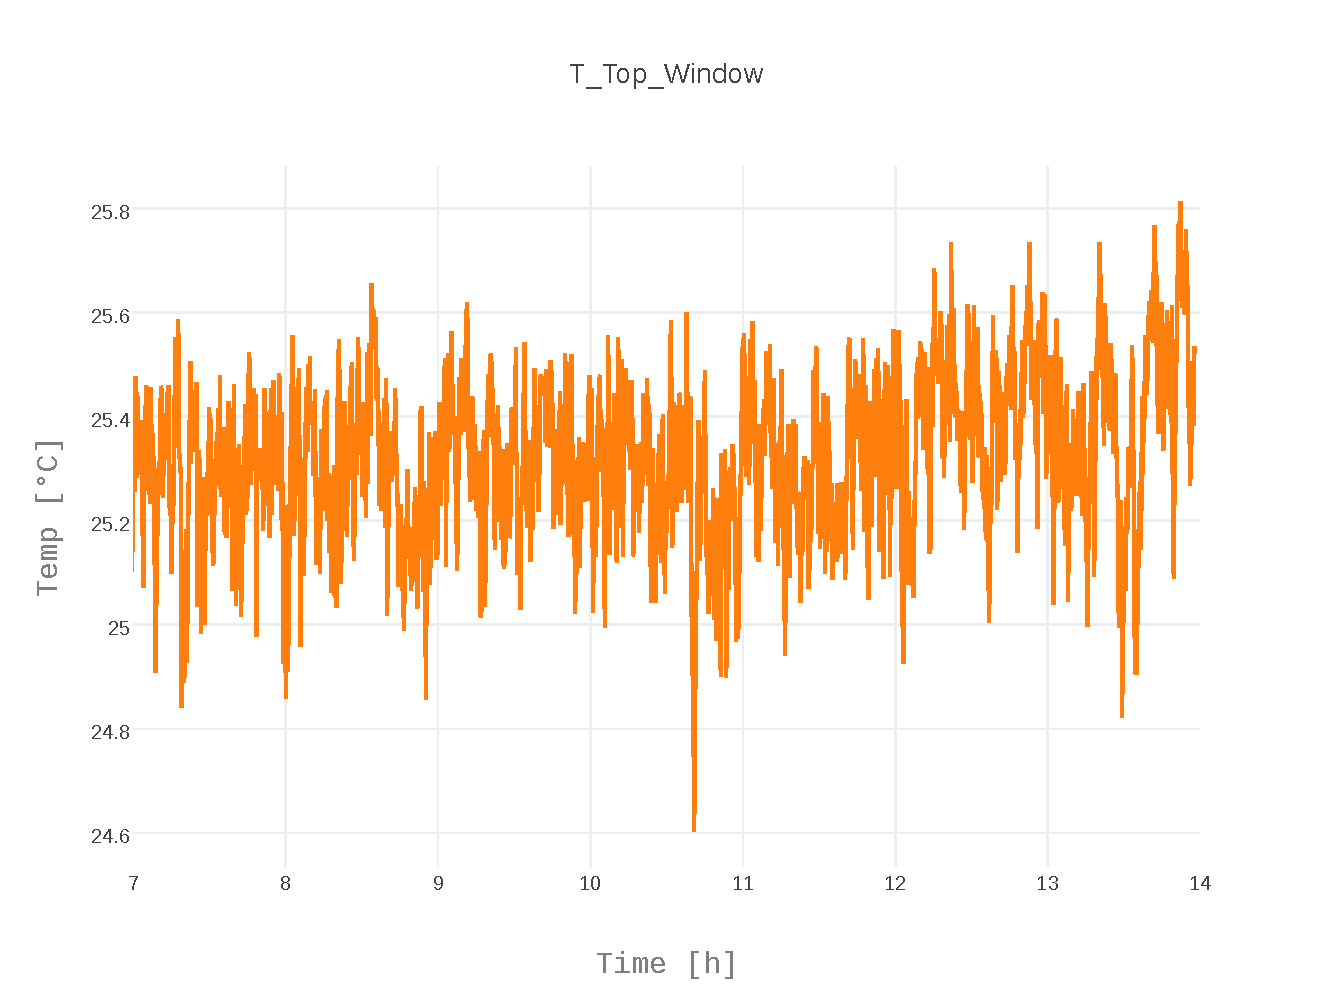
\includegraphics[width = 0.65\textwidth]{./plots/plot_image(20)}}
        \caption{Temperature response to light being turned on}
        \label{fig17}
      \end{figure} \\
      \begin{figure}[h!]
        \hspace{-40pt}
        \subfigure[]{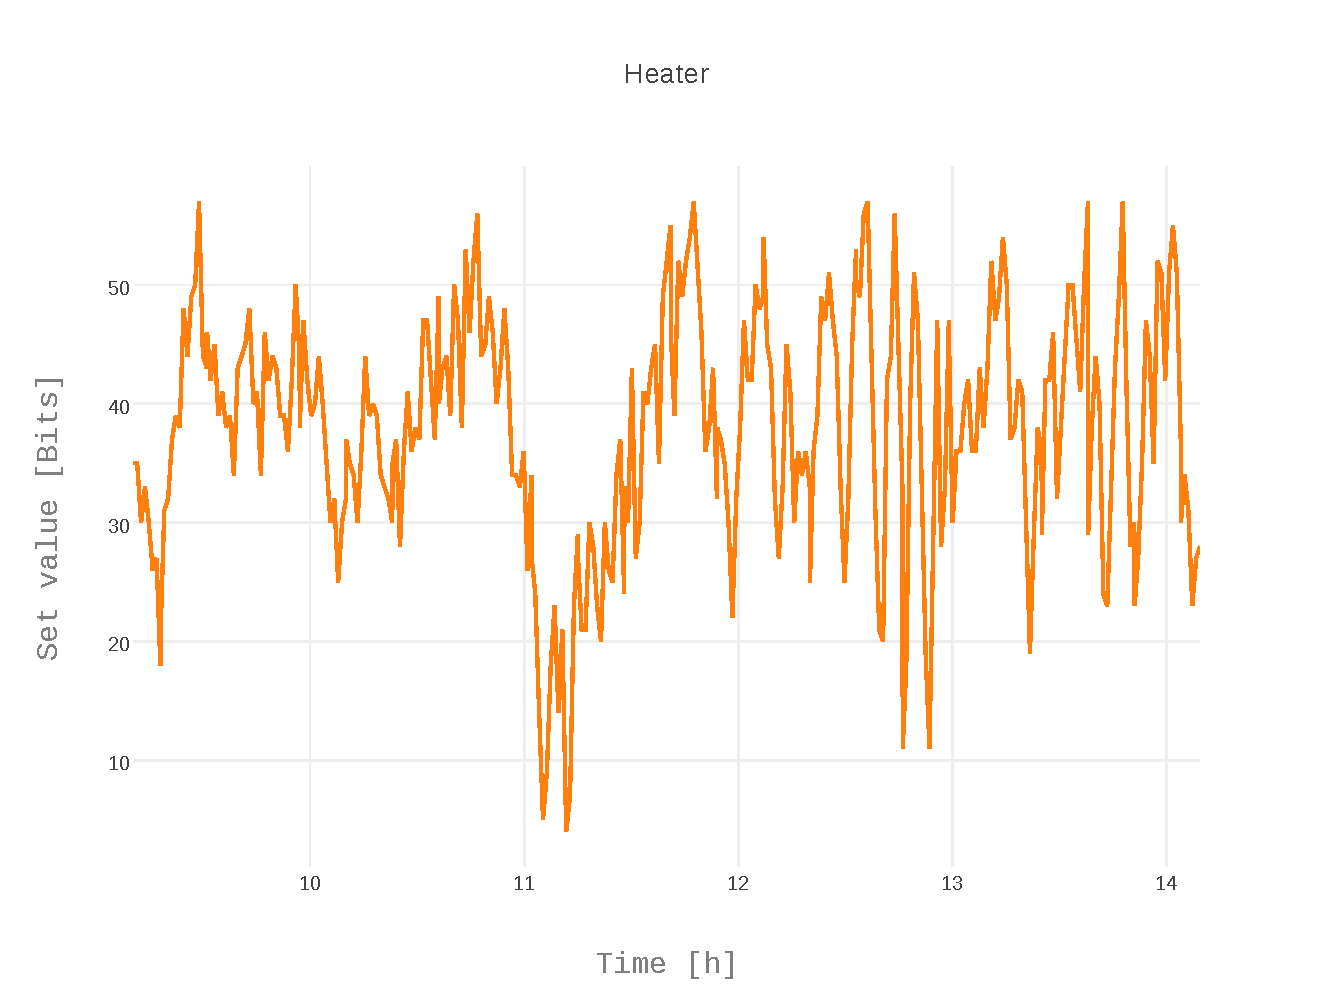
\includegraphics[width = 0.65\textwidth]{./plots/plot_image(21)}}
        \hspace{-20pt}
        \subfigure[]{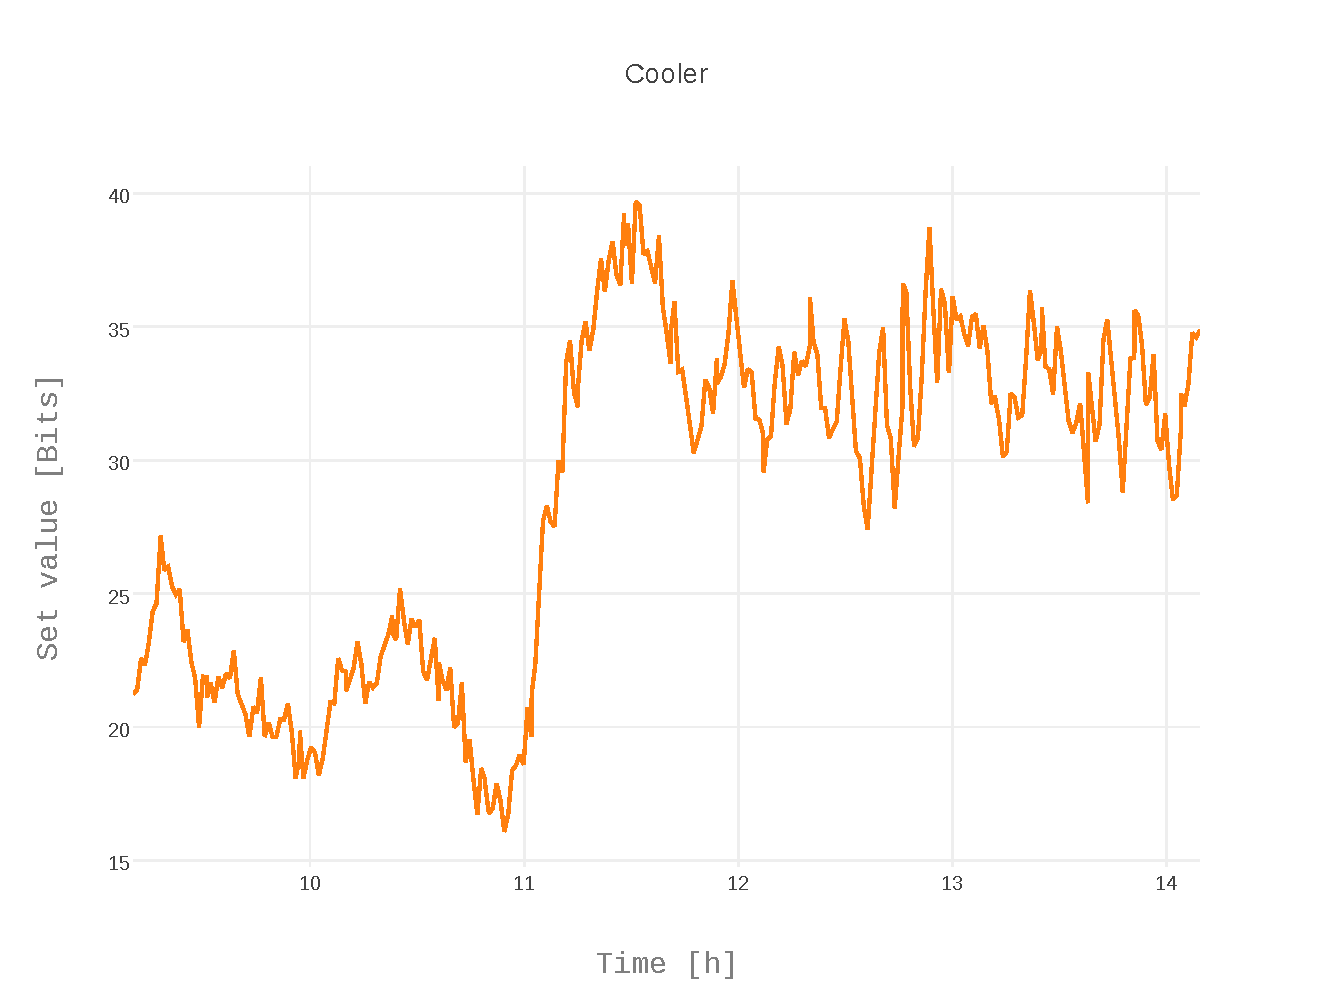
\includegraphics[width = 0.65\textwidth]{./plots/plot_image(22)}}
        \caption{Heater/cooler set values after turning on the lights}
        \label{fig18}
      \end{figure}\\
      \noindent Figure~\ref{fig17} shows that the temperature does oscillate more after
      turning the lights on, especially more to the higher temperatures.
      Below we see that while the heater set value nearly stays the same the
      cooler starts cooling more after turning the lights on.
      \newpage
      \subsubsection{Temperature stabilization over several days}
      Over the weekend of the 24th to 27th I could make a measurement over two
      and a half days. The measurement starts on the 24th at around 16:30 and
      ends at the 27th at around 4:30. Here I can also do a histogram for the
      door and window temperatures, as there is no big jump in them (unlike
      Figure~\ref{fig11}).\\
      From the histograms (Figure~\ref{fig19} (d-f) ) we get the mean and
      standard deviations for the different sensors:
      \\
      \begin{table}[H]
        \begin{tabular}{l | r | r | r}
          & PID & Door & Window \\
          \hline
          $\mu[\text{°C}]$ & $23.514$ & $22.652$ & $24.927$ \\
          $\sigma[\text{K}]$ & $0.075$ & $0.073$ & $0.267$
        \end{tabular}
      \end{table}
      We see that the temperature is fairly stable near the door and the PID
      temperature sensor, with
      not even half a degree deviations. The temperature near the window varies
      more, with a standard deviation of $\sigma = 0.267\,\text{K}$.\\
      Its also visible that the PID sensor seems to show more oscillation on
      daytime and at the window there is a clear rise in temperature over the day.
      \\What can also be seen is that the door temperature seems to be rather
      colder than the mean value, meaning it oscillates more to the cold side
      and the opposite is the case for the window temperature. This can also be
      seen by calculating the weighted difference of points to the right to
      points to the left of the mean. If that number is positive it means that
      we have more points to the left.
      Calculation yields the following values: \vspace{-5pt}
      \begin{table}[H]
        \begin{tabular}{c | c | c}
          PID & Door & Window \\
          \hline
          $9.67\mathrm{e}{-04}$ & $1.77\mathrm{e}{-02}$ & $-1.05\mathrm{e}{-02}$
        \end{tabular}
      \end{table}
      which are consistent with the asumption.
      \begin{figure}[H]
        \hspace{-60pt}
        \subfigure[]{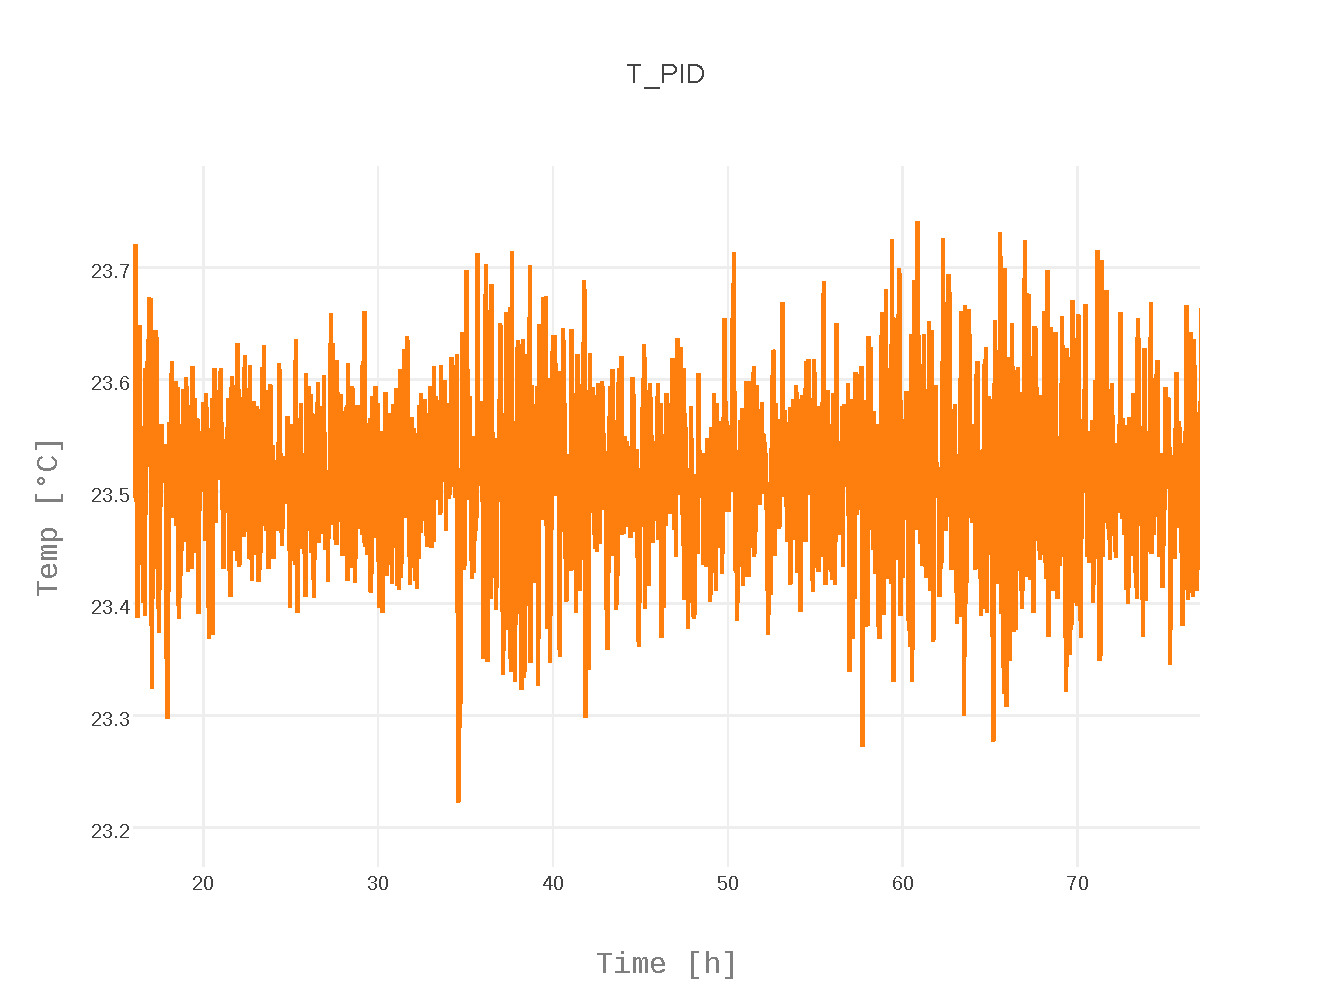
\includegraphics[width = 0.65\textwidth]{./plots/plot_image(23)}}
        \hspace{-20pt}
        \subfigure[]{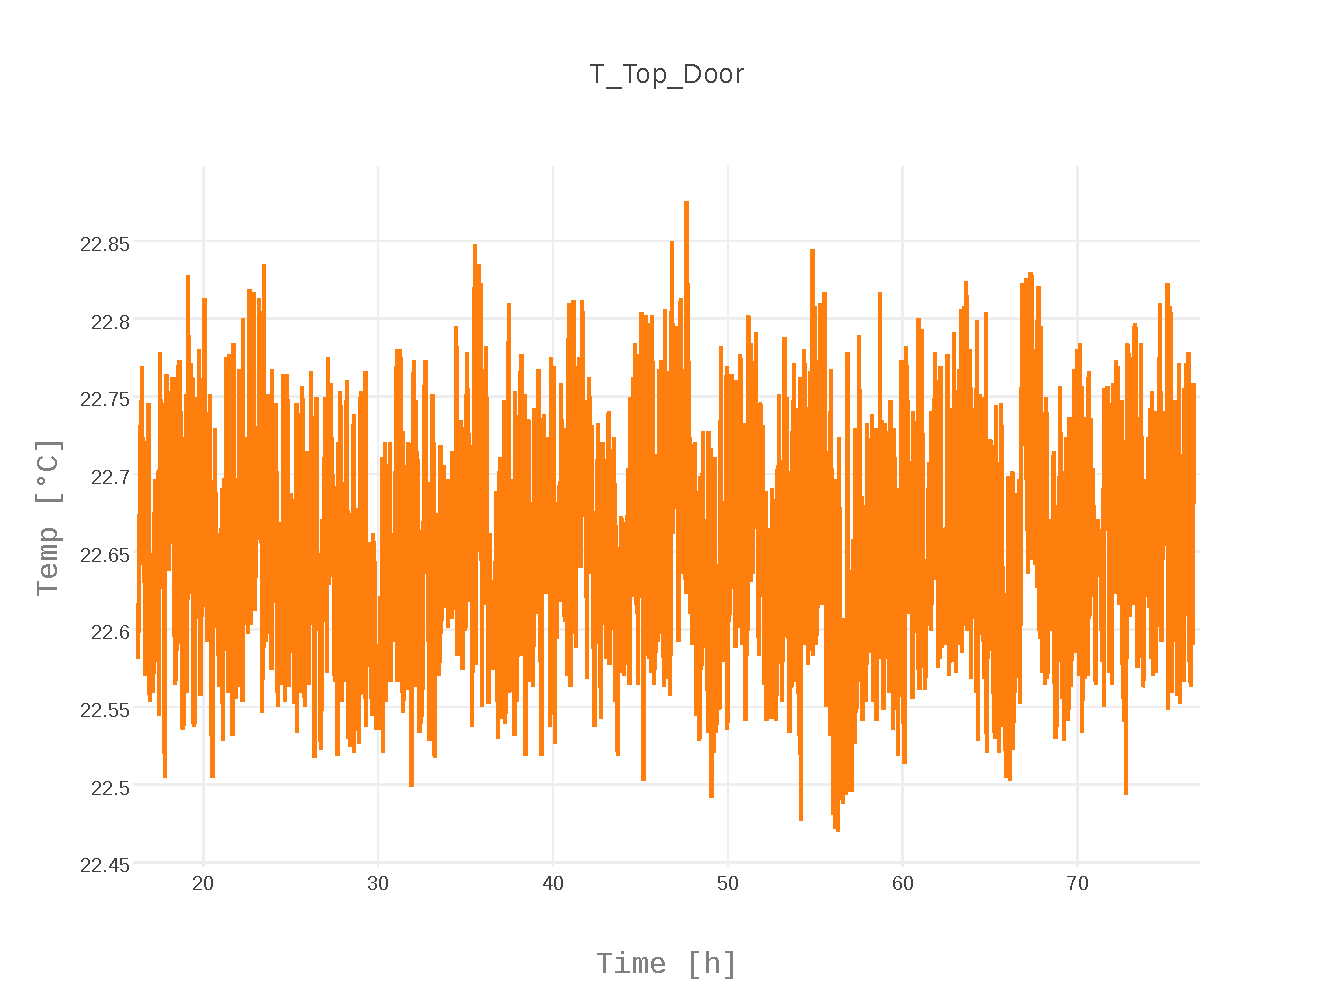
\includegraphics[width = 0.65\textwidth]{./plots/plot_image(24)}}
        \subfigure[]{\hspace{-40pt}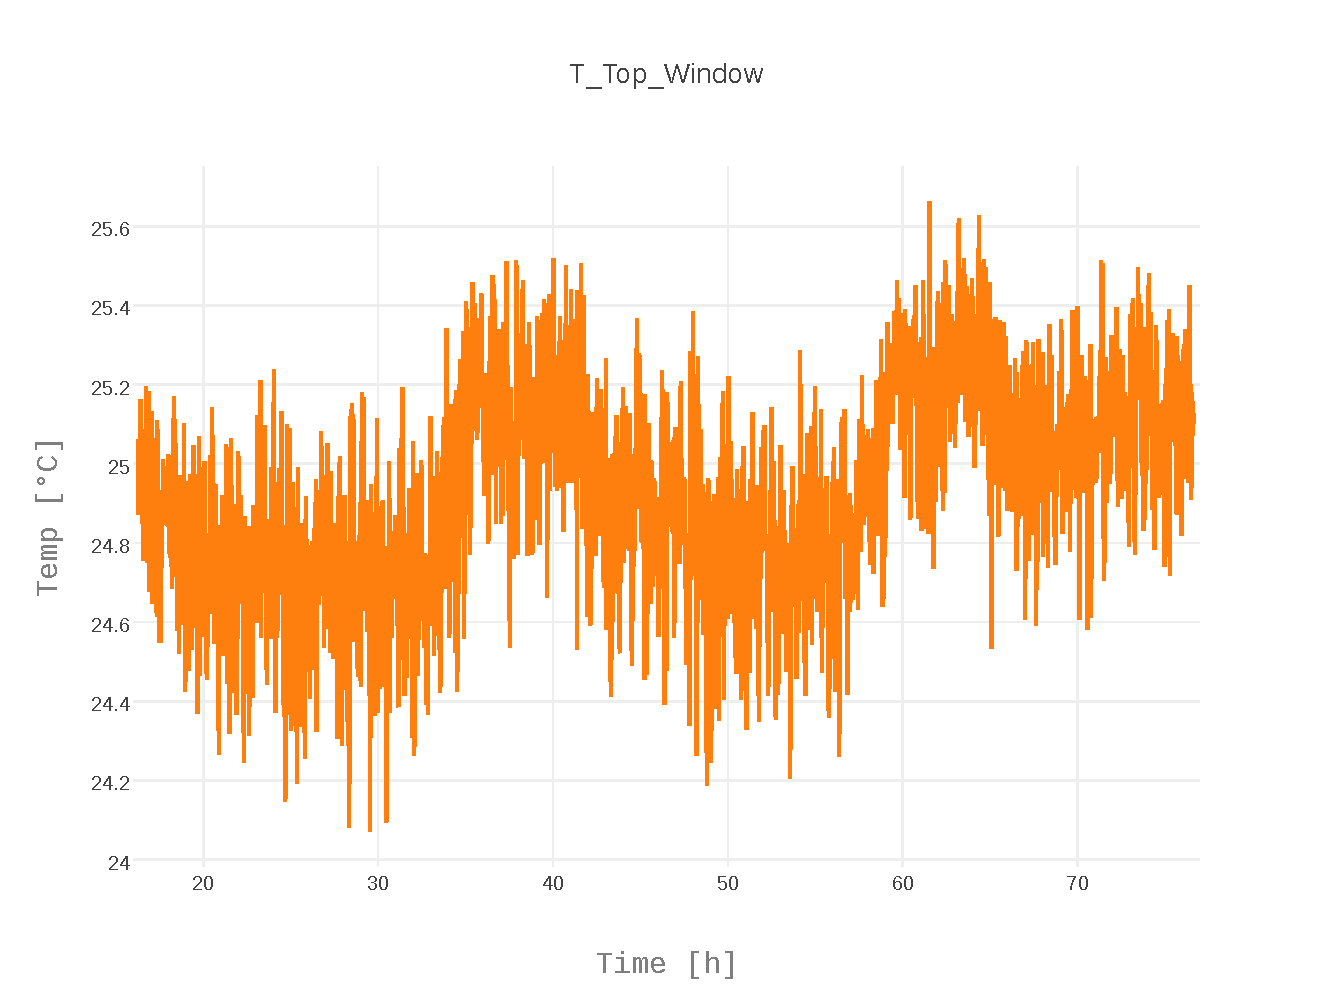
\includegraphics[width = 0.65\textwidth]{./plots/plot_image(25)}}
        \subfigure[]{\hspace{-20pt}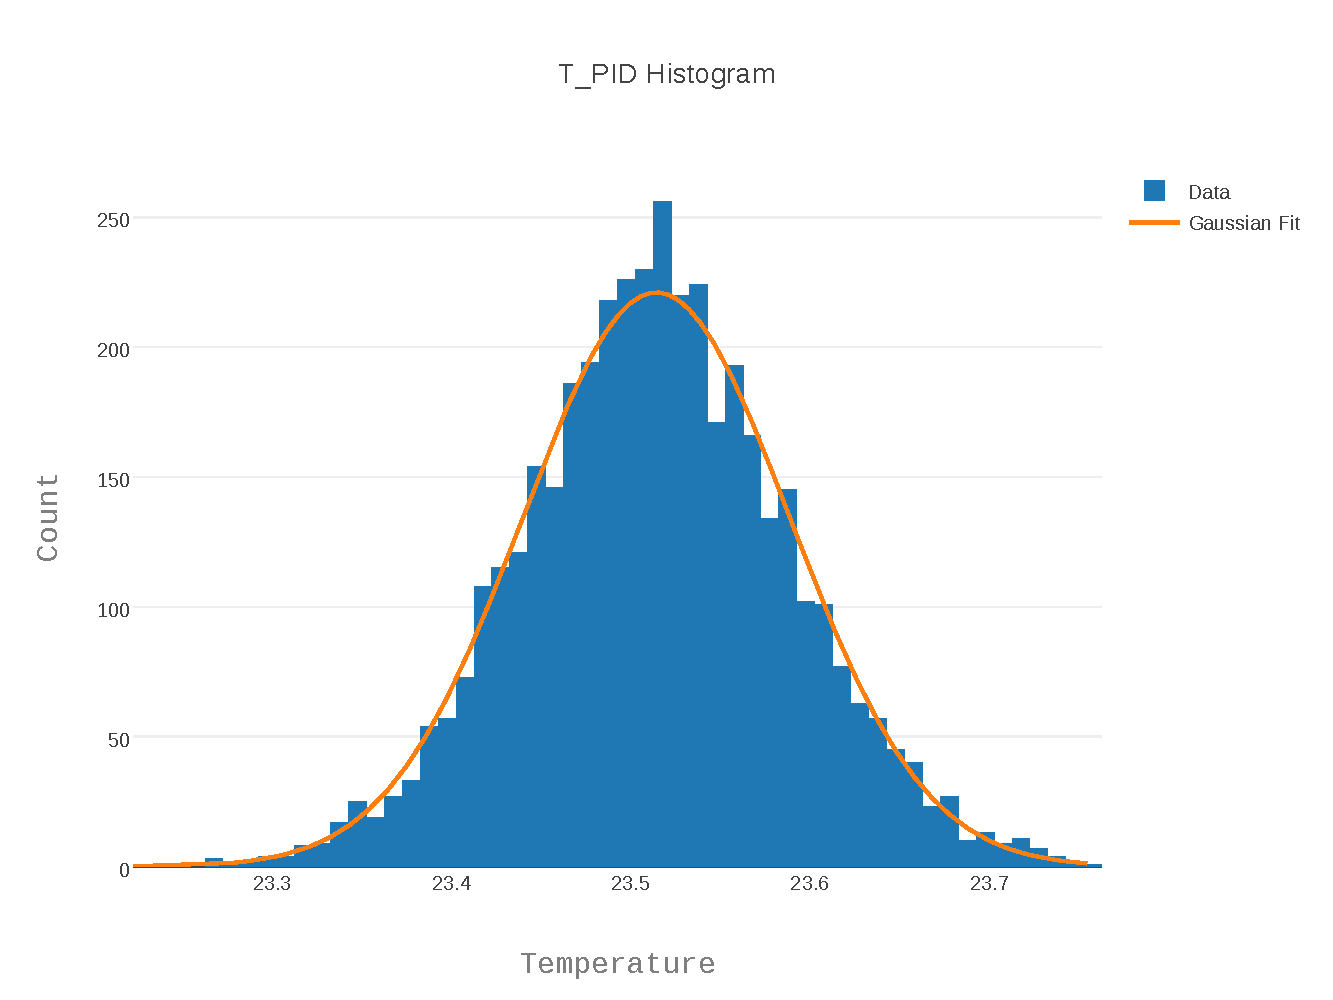
\includegraphics[width = 0.65\textwidth]{./plots/plot_image(26)}}
        \subfigure[]{\hspace{-40pt}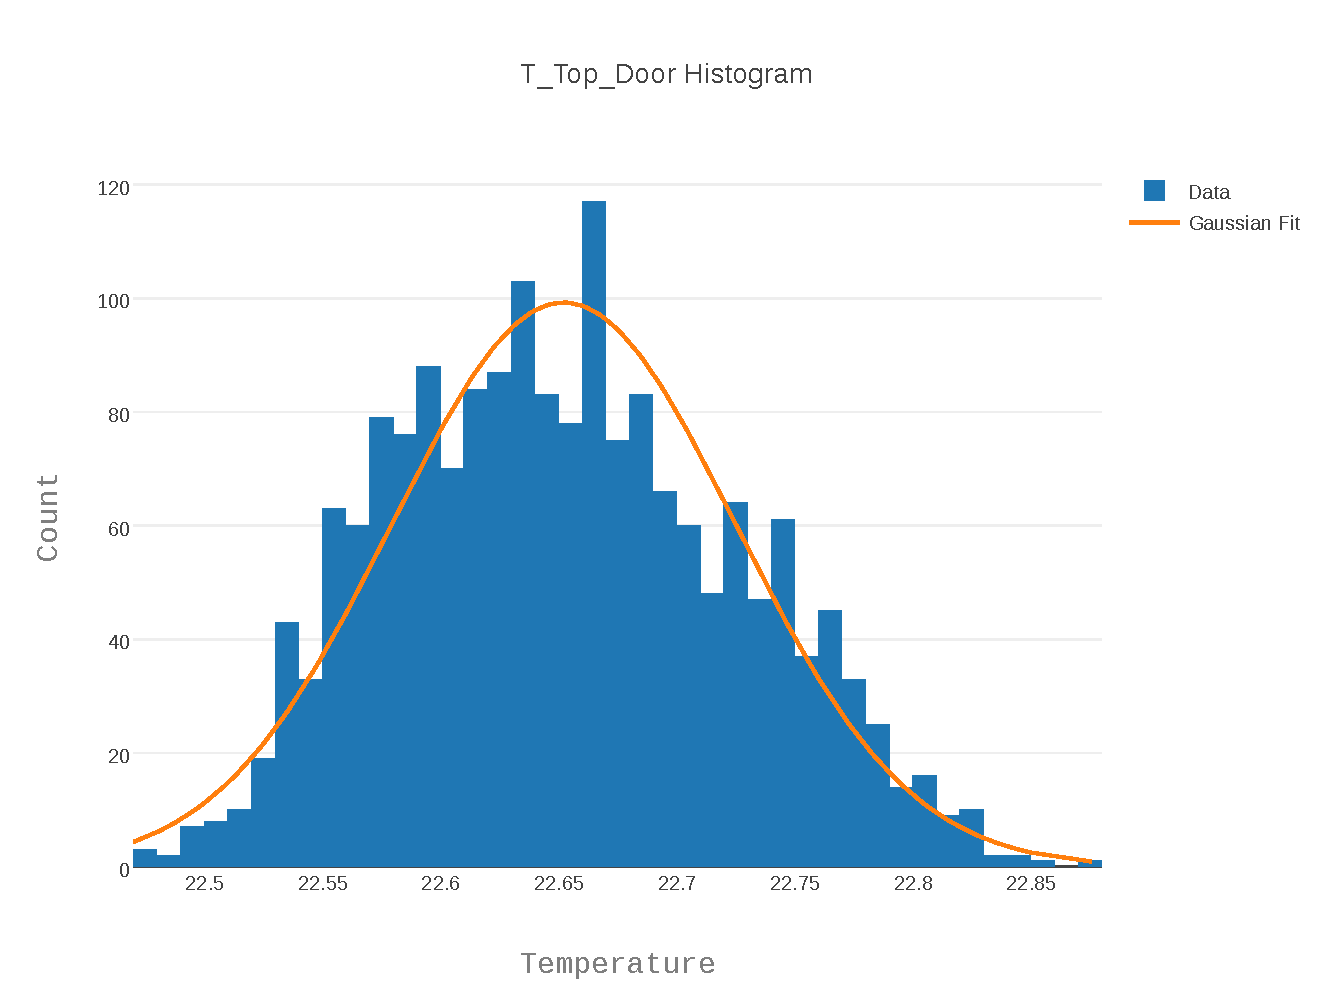
\includegraphics[width = 0.65\textwidth]{./plots/plot_image(27)}}
        \subfigure[]{\hspace{-20pt}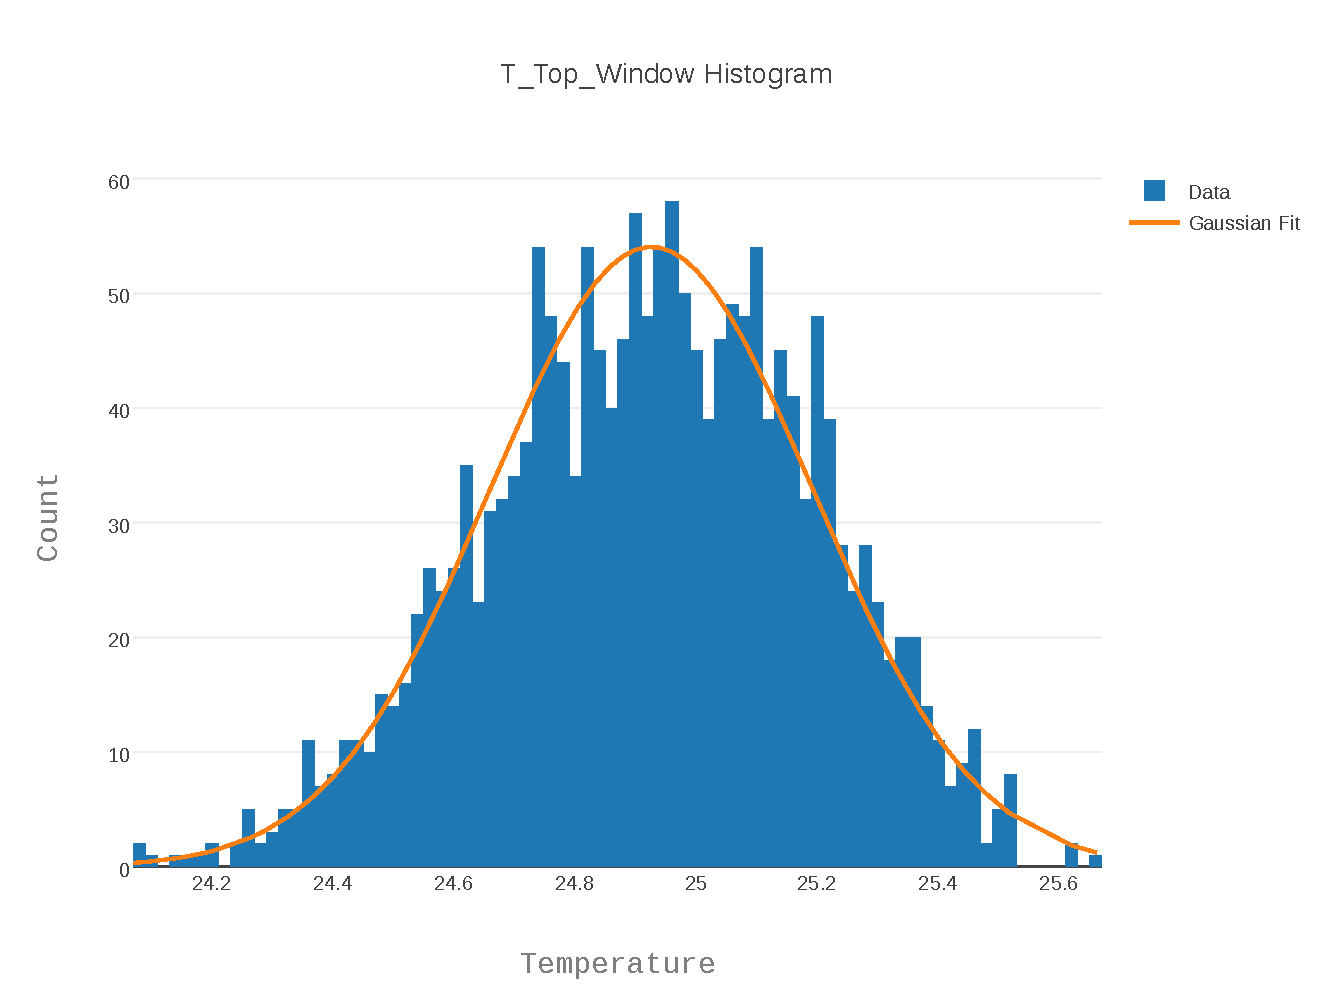
\includegraphics[width = 0.65\textwidth]{./plots/plot_image(28)}}
        \caption{Temperature stabilization over several days with temp. from
        sensors T\_PID, T\_Top\_Door, T\_Top\_Window.}
        \label{fig19}
      \end{figure}

  \section{Overview and discussion}
    I started this project work developing a network interface for the PID
    temperature control system in the control room of the THe-Trap experiment at
    the Max-Planck für Kernphysik.\\
    The temperature control system was originally developed by Vanessa Scheller
    using a Arduino Due platform. I worked with her
    \href{https://www.mpi-hd.mpg.de/THeWiki/index.php/Temperature_stabilization}{log book and report}.\\
    With the original setup it was possible
    to communicate with the Arduino over the serial interface, but only with a
    computer connected over the USB-port. To ensure a connection over the local
    network the most straightforward attempt was installing a Ethernet Shield on
    top of the Arduino (Figure~\ref{fig6}). With this it is possible to get
    information from the Arduino using a socket communication over a local port.
    It was not however possible to directly write the data from the Arduino on
    a network device. The data is send from the Arduino upon request to a handling
    script on a local computer. The controlling script is described in
    \nameref{sec:control}.\\
    The network communication could also have been realized using a small
    single-board computer such as the Raspberry Pi. With this it would have been
    possible to directly save to data on the network drive and control the PID
    with commands send to the single-board computer. The disadvantage is that
    this would make the system more complex and probably more prone to errors.\\
    I continued with reworking the level shifting circuits for the temperature
    input and heater/cooler set value output. I worked with the schematics from
    the previous setup and designed a circuit board which could then be realized
    with a circuit board mill (Figure~\ref{fig4},~\ref{fig5}). The new
    level shifter board should be more failsafe and it also leads to a much
    tidier setup, because it also fits into the same enclosure as the Arduino
    board (Figure~\ref{fig7}).
    The complete schematics from Vanessa Scheller are shown in Figure~\ref{fig20}.
    I also used the same resistance values for the resistors for the
    \hyperref[tempres]{temperature} and the \hyperref[hcres]{heater/cooler}
    shifter circuit.\\
    With the network interface I was also abled to do a more thourough testing
    of the temperature control than before. The temperature control system
    should of course hold the temperature as constant as possible under
    influences that would change the temperature, such as change in daytime
    temperature. I used three different sensor which were placed at different
    spots in the control room. The temperature near the door showed a very
    good constant temperature behaviour ($\sigma = 0.073\,\text{K}$), the
    temperature near the window does oscillate a little bit more with
    $\sigma = 0.267\,\text{K}$ (Figure~\ref{fig19}). \\
    With changing the temperature reference I could examine the behaviour for a
    rapid change in temperature. With this one can get a good estimate for the
    time it takes for the system to regulate back to the reference temperature.
    I calculated time constants which are circa 30 minutes for a change of
    about $1.3$~K , depending on the time of the day and the sensor placement
    (Figure~12-16).\\
    I also tested the influence of turning the lights on in the control room.
    The influence on the temperature is visible as bigger oscillation on the
    sensors (Figure~\ref{fig17}) and as a higher cooler set value from the PID
    (Figure~\ref{fig18}). The change in temperature is still rather small.\\
    One thing which the temperature control system could not prevent is a temperature
    gradient over the room, as it only controls towards the temperature at one
    fixed place in the room. This can be seen in Figure~\ref{fig11}. Here the
    temperature near the door and the window make a fast change probably due to
    local change in temperature (i.e. light from the window) and are not regulated
    back, but stay at the higher/lower level. This effect was probably increased
    by the placement of the heater and cooler systems, with the heater being
    near the window and the cooler being near the door.\\
    Concluding it can be said, that the PID temperature control system works
    fairly well and can also withstand influences such as change in outside
    temperature, lights being turned on and a rapid change in temperature, but
    it can happen that it builds up a temperature gradient. Whether or not this
    drawback does actually influence the results of the experiment (or whether the temperature control is at all
    necessary) remains to be seen.

  \section{Appendix}
    \begin{figure}[h!]
      \centering
      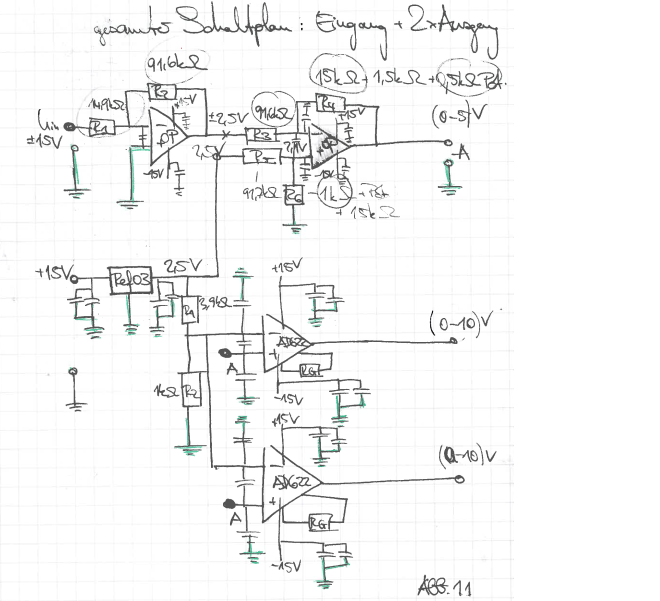
\includegraphics[width = \textwidth]{schaltplanvan.png}
      \caption{Circuit board schematics from Vanessa Scheller}
      \label{fig20}
    \end{figure}
\end{document}
